\documentclass[final]{siamltex}

% Be sure to use PDF Latex
\pdfoutput=1

\usepackage[latin1]{inputenc}
\usepackage{array}% http://ctan.org/pkg/array
\usepackage{rotating}
\usepackage{graphicx,cancel}
%\usepackage{pdfsync}
\usepackage{epsfig,hyperref}
% \usepackage{movie15,animate}
\usepackage{epstopdf}
\usepackage{mystyle,ulem}
\usepackage{color}
% format A4
\usepackage{vmargin}
\setpapersize{A4} 

\usepackage{color}
\newcommand{\red}{\color{red}}
\newcommand{\todo}[1]{{\color{red} TODO: #1}}

\newcommand{\now}[1]{{\color{blue} NOW: #1}}
\newcommand{\before}[1]{{\color{red} BEFORE: #1}}


\author{Nicolas Papadakis\thanks{IMB, Universit\'e Bordeaux 1, 351, cours de la Lib\'eration, F-33405 TALENCE, FRANCE.}
\and Gabriel Peyr\'e\thanks{CEREMADE, Universit\'e Paris-Dauphine, Place du Marechal De Lattre De Tassigny, 75775 PARIS CEDEX 16, FRANCE.}
\and Edouard Oudet\thanks{LJK, Universit\'e de Grenoble, 51 rue des Math\'ematiques, Campus de Saint Martin d'H\`eres, BP 53, 38041 GRENOBLE CEDEX 09}
}


\graphicspath{{./images/}}

\if 0
\orderauthors{1}%\NewRandom}
\author{\listauthors{\auta}
	 \quad \listauthors{\autb}\\\\
	 \quad \listauthors{\autc}
	\
}
\fi

\title{Optimal Transport with  Proximal Splitting}



%%%%%%%%%%%%%%%%%%%%%%%%%%%%%%%%%%%%%%%%%%%%%%%%%%%%%%%%%%%%%%%%
\begin{document}

\maketitle

% \if 0
\begin{abstract}
	This article reviews the use of first order convex optimization schemes to solve the discretized dynamic optimal transport problem, initially proposed by Benamou and Brenier. We develop a staggered grid discretization that is well adapted to the computation of the $L^2$ optimal transport geodesic between distributions defined on a uniform spatial grid. We show how proximal splitting schemes can be used to solve the resulting large scale convex optimization problem. A specific instantiation of this method on a centered grid corresponds to the initial algorithm developed by Benamou and Brenier. We also show how more general cost functions can be taken into account and how to extend the method to perform optimal transport on a Riemannian manifold. 
\end{abstract}

\begin{keywords}Optimal transport, proximal splitting, Douglas-Rachford, ADMM, primal-dual.\end{keywords}

\begin{AMS}90C25, 68U10\end{AMS}


%%%%%%%%%%%%%%%%%%%%%%%%%%%%%%%%%%%%%%%%%%%%%%%%%%%%%%%%%%%%%%
%%%%%%%%%%%%%%%%%%%%%%%%%%%%%%%%%%%%%%%%%%%%%%%%%%%%%%%%%%%%%%%%
\section{Introduction}


Optimal transport is a well developed mathematical theory that defines a family of metrics between probability distributions~\cite{Villani03}. These metrics measure the amplitude of an optimal displacement according to a so-called ground cost defined on the space supporting the distributions. The resulting distance is sometimes referred to as the Wasserstein distance in the case of $L^p$ ground costs. The geometric nature of optimal transportation, as well as the ability to compute optimal displacements between densities, make this theory progressively mainstream in several applicative fields such as economic modeling and image processing. However, the numerical resolution of the optimal transportation problem raises several challenges. This article is focused on the  computation of geodesics for the optimal transport metric associated to the $L^2$ cost. It reviews and extends the approach pioneered by Benamou and Brenier~\cite{Benamou2000} from the perspective of proximal operator splitting in convex optimization. This shows the simplicity and efficiency of this method, which can easily be extended beyond the setting of optimal transport by considering various convex cost functions.

%%%%%%%%%%%%%%%%%%%%%%%%%%%%%%%%%%%%%%%%%%%%%%%%%%%%%%%%%%%%%%
\subsection{Previous Works} 
\label{sec-previous}


%%%
\paragraph{Discrete optimal transport}

The easiest way to discretize and compute numerically optimal transports is to consider finite sums of weighted Diracs. In this specific case, the optimal transport is a multi-valued map between the Diracs locations. % and it is the solution of a linear program. 
 Specific linear solvers can be used in this context, and in particular network and transportation simplexes~\cite{Dantzig-Book} can scale up to a few thousands of Dirac masses. Dedicated combinatorial optimization methods have been proposed, such as the auction algorithm~\cite{Bertsekas1988}, which can handle integer costs between the Diracs. In the even more restricted case of two distributions with the same number of Diracs with equal weights, the transportation is a bijection between the points, and thus corresponds to the optimal assignment problem~\cite{Burkard09}. Combinatorial optimization methods such as the Hungarian algorithm~\cite{Kuhn-hungarian} have roughly cubic complexity in the number of Diracs. Faster schemes exist for specific cost functions, such as for instance convex cost of the distance on the line (where it boils down to a sorting of the positions) and the circle~\cite{delon-circle}, concave costs on the line~\cite{delon-concave}, the $\ell^1$ distance~\cite{Ling2007}. The computation can be accelerated using multi-scale clustering~\cite{Merigot2011}. Note also that various approximations of the transportation distance have been proposed, see for instance~\cite{Shirdhonkar2008}.

Despite being numerically intensive for finely discretized distributions, this discrete transport framework have found many applications, such as for instance color transfer between images~\cite{Rabin2011}, shape retrieval~\cite{Rubner1998}, surface reconstruction~\cite{deGoes2011} and interpolation for computer graphics~\cite{Bonneel-displacement}


%%%
\medskip
\paragraph{Optimal transport via PDE's}

The optimal transport for the $L^2$ ground cost has a special structure. It can be shown to be uniquely defined and to be the gradient of a convex function~\cite{Brenier1991}. This implies that it is also the solution of the fully non-linear Monge-Amp\`ere partial differential equation.

% --- PDE Monge ampere ---

Several methods have been proposed to discretize and solve this PDE, such as for instance the method of~\cite{Oliker-Prussner-1988} which converges to the Aleksandrov solution, and the one of~\cite{Oberman-2008} which converges to the viscosity solution of the equation. Alternative methods such as~\cite{Dean-Glowinski-2006} and~\cite{Feng-Neilan-2009} are efficient for regular densities.  A major difficulty in these approaches is to deal with compactly supported densities, which requires a careful handing of the boundary conditions. \cite{Froese2012} proposes to enforce these conditions by iteratively solving a Monge-Ampere equation with Neumann boundary conditions. \cite{Benamou2012} introduces a method requiring the solution of a well-posed Hamilton-Jacobi equation.

% --- AHT et cie --

Another line of methods iteratively constructs mass preserving mappings converging to the optimal transport~\cite{Angenent2003}. This explicitly constructs the so-called polar factorization of the initial map, see also~\cite{Benamou1995} for a different approach. This method is enhanced in~\cite{Haber2010} to avoid drifting from the preservation constraint during the iterations.

% --- AHT et cie --


These PDE's based approaches to the resolution of the optimal transport have found several applications,  such as image registration~\cite{haker2004}, density regularization~\cite{Burger2011}, optical flow~\cite{Clarysse2010} and grid generation~\cite{Sulman2011b}.

% Citations enlev�es : 
%~\cite{Kitagawa2012} -> the cost is not necessarily L^2, not in R^d ... A bit weird. 
%~\cite{Loeper2005}  : juste un newton sur l'EDP ... ne me semble pas tr�s s�rieux.
%~\cite{Sulman2011} (M. Sulman, J. F. Williams, and Robert D. Russell. An efficient approach for the numerical solution of the monge-amp`ere equation.) : je n'y ai pas acc�s



%%%
\medskip
\paragraph{Dynamical optimal transport}

Instead of computing directly the transport, it is possible to consider the geodesic path between the two densities according to the Wasserstein metric (the so-called displacement interpolation). For the $L^2$ ground cost, this geodesic is obtained by linear interpolation between the identity and the transport. The geodesic can thus be computed by first obtaining the transport and then evolving the densities. If one considers discrete sums of Diracs, this corresponds to solving a convex linear program, and can also be understood as a Lagrangian approximation of the transport between (possibly continuous) densities that have been discretized. This approach is refined in~\cite{Iollo2011}, which considers discretization with mixture of Gaussians.

It is also possible to consider an Eulerian formulation of the geodesic problem, for which densities along the path are discretized on a fixed spatial grid. Conservation of mass is achieved by introducing an incompressible velocity field transporting the densities. The breakthrough paper~\cite{Benamou2000} shows that it is possible to perform a change of variable to obtain a convex problem. They propose to solve numerically the discretized problem with a first order iterative method (more precisely, they use the ADMM algorithm on a dual formulation, see bellow).

Geodesics between pairs of distributions can be extended to barycenters between an arbitrary finite collection of distributions. Existence and uniqueness of this barycenter is studied in~\cite{Carlier_wasserstein_barycenter}. Computing the barycenter between discrete distributions requires the resolution of a convex linear program that corresponds to a multi-marginal optimal transportation. However, in sharp contrast with the case of two distributions, the special case of un-weighted sums of Diracs is not anymore equivalent to an assignment problem, which is known to be NP-hard~\cite{Burkard09}. Computing numerically this barycenter for large scale problems thus requires the use of a non-convex formulation to solve for a Lagrangian discretization, which finds applications in image processing~\cite{Rabin_ssvm11}.


%%%
\medskip
\paragraph{Generalized transport problems}

The formulation of the geodesic computation as a convex optimization problem initiated by~\cite{Benamou2000} enables the definition of various metrics obtained by changing the objective function. A penalization of the matching constraint~\cite{Benamou2010} allows one to compute an unbalanced transport where densities are not normalized to have the same mass. An interpolation between the $L^2$-Wasserstein and $L^2$ distances is proposed in~\cite{Benamou2001}. Lastly, an interpolation between $L^2$-Wasserstein and $H^{-1}$ distances is described in~\cite{dolbeault2009}. This extension relies in a crucial manner on the convexity of the extended objective function, which enables a theoretical analysis to characterize minimizing geodesics~\cite{Cardaliaguet2012}. Convexity also allows one to use the numerical scheme we propose with only slight modifications with respect to the $L^2$-Wasserstein case. 

%%%
\medskip
\paragraph{Optimal transport on Riemannian manifolds}

Many properties of the $L^2$-Was\-ser\-stein distance extend to the setting where the ground cost is the square of the geodesic distance on a Riemannian manifold. This includes in particular the existence and uniqueness of the transport map, which is the manifold exponential of the gradient of a semi-convex map~\cite{McCann-PolarManifold}. Displacement interpolation for transport on manifolds has the same variational characterization as the one introduced in~\cite{Benamou2001} for Euclidean transport, see~\cite{Villani-OldNew} for a detailed review of optimal transport on manifolds. Interpolation between pairs of measures generalizes to barycenters of a family of measures, see~\cite{KimPass-MultiMarg-Manifold}.

Displacement interpolation between Dirac measures amounts to computing a single geodesic curve on the manifold. Discretization and numerical solutions to this problem are numerous. A popular method is the Fast Marching algorithm introduced jointly by~\cite{sethianFM1995,tsitsiklis-TAC} for isotropic Riemannian metrics (i.e. when the metric at each point is a scalar multiple of the identity) discretized on a rectangular grid. The complexity of the method is $O(N \log(N))$ operations, where $N$ is the number of grid points. This algorithm has been extended to compute geodesics on 2-D triangular meshes with only acute angles~\cite{sethian-geodesic-path}. More general discretizations and the extension to Finsler metrics require the use of slower iterative schemes, see for instance~\cite{bornemann-fm}. 

Computing numerically optimal transport on manifolds has been less studied. For weighted sums of Diracs, displacement interpolation is achieved by solving the linear program to compute the coupling between the Diracs and then advancing the Diracs with the corresponding weights and constant velocity along the geodesics. In this article, we propose to extend the Eulerian discretization method~\cite{Benamou2001} to solve for the displacement interpolation on a Riemannian manifold.

%%%
\medskip
\paragraph{First order and proximal methods}

The convex problem considered by Benamou and Brenier~\cite{Benamou2000} can be re-casted as the optimization of a linear  functional under second order conic constraints (see Section~\ref{sec-socp} for more details). This class of programs can be solved in time polynomial with the desired accuracy using interior points methods, see for instance~\cite{Nesterov-Nemirovsky-Book}. 

However, the special structure of the problem, specially when discretized on an uniform grid, makes its suitable for first order scheme, and in particular proximal splitting methods. While they do not reach the same convergence speed for arbitrary conic program, they work well in practice for large scale problems, in particular when high accuracy is not mandatory, which is a common setup for problems in image processing. Proximal splitting schemes are first order optimization methods that allows one to minimize a sum of so-called ``simple'' functionals, possibly (for some methods) pre-composed by linear operators. A functional is called ``simple'' when it is possible to compute its proximal operator (see expression~\ref{eq:def_prox} for its precise definition) either in closed form, or with high accuracy using a few iterations of some sub-routine. In this article, we focus our attention to the Douglas-Rachford algorithm, introduced by~\cite{Lions-Mercier-DR} and on primal-dual methods. We make use of the recently proposed method~\cite{Chambolle2011}, but other schemes could be used as well, see for instance~\cite{Briceno-Arias-PD}. We refer the reader to~\cite{combettes-pesquet-review} and the references therein for more information about the properties of proximal maps and the associated proximal splitting schemes. 

Note that the algorithm proposed by~\cite{Benamou2000} corresponds to applying the  Alternating Direction Method of Multiplier (ADDM)~\cite{Fortin1983} to the Fenchel-Rockafeller dual of the (primal) dynamical transport problem. As shown by~\cite{Eckstein1992}, this corresponds exactly to applying directly (a specific instanciation of) the Douglas-Rachford method to the primal problem. 

%%%
\medskip
\paragraph{Fluid mechanics discretization}

While Lagrangian methods utilize a mesh-free discretizations (see for instance~\cite{Iollo2011}), thats typically tracks the movement of centers of masses during the transportation, Eulerian method requires a fixed discretization of the spacial domain. The most straightforward strategy is to use an uniform centered discretization of an axis-aligned domain, which is used in most previously cited work, see for instance~\cite{Benamou2000,Angenent2003}. Because of the close connection between dynamical optimal transport and fluid dynamics, we advocate in this article the use of staggered grids~\cite{anderson-cfd}, which better copes with the incompressibility condition. 



%%%%%%%%%%%%%%%%%%%%%%%%%%%%%%%%%%%%%%%%%%%%%%%%%%%%%%%%%%%%%%
\subsection{Contributions}

Our first contribution is to show how the method initially proposed in~\cite{Benamou2000} is a specific instance of the Douglas-Rachford algorithm. This allows one to use several variations on the initial method, by changing the values of the two relaxation parameters. Our second contribution is the introduction of a staggered grid discretization which is the canonical way to enforce incompressibility constraints. We show how this discretization  fits into our proximal splitting methodology by introducing an interpolation operator and either making use of auxiliary variables or primal-dual methods. Our last contribution includes an exploration of several variations on the original convex transportation objective, the one proposed in~\cite{dolbeault2009}, and a specially varying penalization which can be interpreted as replacing the $L^2$ ground cost by a geodesic distance on a Riemannian manifold.  Note that the Matlab source code to reproduce the figures of this article is available online\footnote{\url{http://www.ceremade.dauphine.fr/~peyre/codes/}}.

%%%%%%%%%%%%%%%%%%%%%%%%%%%%%%%%%%%%%%%%%%%%%%%%%%%%%%%%%%%%%%
% \subsection{Notations}




%%%%%%%%%%%%%%%%%%%%%%%%%%%%%%%%%%%%%%%%%%%%%%%%%%%%%%%%%%%%%%
%%%%%%%%%%%%%%%%%%%%%%%%%%%%%%%%%%%%%%%%%%%%%%%%%%%%%%%%%%%%%%%%
\section{Dynamical Optimal Transport Formulation}


%%%%%%%%%%%%%%%%%%%%%%%%%%%%%%%%%%%%%%%%%%%%%%%%%%%%%%%%%%%%%%
\subsection{Optimal Transport}

In the following, we restrict our exposition to smooth maps $T : [0,1]^d \mapsto [0,1]^d$ where $d>0$ is the dimension of the problem. A valid transport map $T$ is a map that  pushes forward the measure $f^0(x) \d x$ onto $f^1(x) \d x$. In term of densities, this corresponds to
the constraint
\eq{ 
	f^0(x) = f^1(T(x)) \abs{\det( \partial T(x) )} 
}
where $\partial T(x) \in \RR^{d \times d}$ is the differential of $T$
at $x$. This is known as the gradient equation. We call $\Tt(f^0,f^1)$ the set of transport that satisfies this constraint.
An optimal transport $T$ solves
\eql{\label{eq-ot} 
	\umin{T \in \Tt(f^0,f^1) } \int C(x,T(x)) \d x 
}
where $C(x,y) \geq 0$ is the cost of assigning $x \in [0,1]^d$ to $y \in [0,1]^d$. 
In the case $C(x,y)=\norm{x-y}^2$, the optimal value of~\eqref{eq-ot}, the so-called optimal transport distance, is often called the  $L^2$-Wasserstein distance between the densities $f^0$ and $f^1$.


%%%%%%%%%%%%%%%%%%%%%%%%%%%%%%%%%%%%%%%%%%%%%%%%%%%%%%%%%%%%%%
\subsection{Fluid Mechanics Formulation}

The geodesic path between the measures with densities $f^0(x)$ and $f^1(x)$ can be shown to have density $t \mapsto f(x,t)$ where $t \in [0,1]$ parameterizes the path, where 
\eq{ 
	f(x,t) = f^0( T_t(x) ) 
   \abs{\det( \partial T_t(x) )}
   \qwhereq 
   T_t = (1-t) \text{Id}_d + t T. 
} 
Benamou and Brenier showed in~\cite{Benamou2000} that this geodesic solves the following 
non-convex problem over the densities $f(x,t) \in \RR$ and a velocity field $v(x,t) \in \RR^2$
\eql{\label{eq-bb-continuous_velocity} 
	\umin{ (v,f) \in \Cinc^0 } \frac12\int_{[0,1]^d} \int_0^1 f(x,t)\norm{v(x,t)}^2 \d t \d x, 
}
under the set of non-linear constraints
\eql{\label{eq-inc-constr} 
	\Cinc^0 = \enscond{(v,f)}{\partial_t f+ \diverg_x(fv) = 0, 
      \;  v(0,\cdot)=v(1,\cdot)=0, \;  f(\cdot,0)=f^0, \;  f(\cdot,1)=f^1  }. 
}
where the first relation in $\Cinc^0$ is the continuity equation. We impose homogeneous Neumann conditions on the velocity field $v$ which are the more natural boundary condition in the case of the square. Notice that both Neumann and Dirichlet boundary conditions can easily be implemented in our framework. The difference relies in the projection step on the divergence constraint. This step which is carried out using the Fast Fourier Transform algorithm, has to be adapted depending on the chosen boundary conditions.  We refer to~\cite{Froese2012,Benamou2012} for relevant boundary conditions for other convex geometries. The temporal boundary constraints on $f$ impose a match with the input density data.

From a theoretical point of view, the natural setting to prove existence of minimizers of~\eqref{eq-bb-continuous_velocity} is to relax the variational problem and perform the optimization over the Banach space of Radon measures (i.e. finite Borel measures). It is a sub-space of the space of distributions and the incompressibility constraint~\eqref{eq-inc-constr} should be understood in the sense of distributions. We refer the interested reader to~\cite{Cardaliaguet2012} for more details regarding the theoretical analysis of a class of variational problems generalizing~\eqref{eq-bb-continuous_velocity}.  

Note that once an optimal vector field $v$ solving~\eqref{eq-bb-continuous_velocity} has been computed, it is possible to recover an optimal transport $T$ by integrating the flow in time. From a given $x \in [0,1]^d$, we define the solution $t \mapsto T_t(x)$ solving 
\eq{
	T_0(x) = x
	\qandq
	\foralls t > 0, \quad \pd{T_t(x)}{t} = v( T_t(x), t ).
}
The optimal transport is then obtained at $t=1$, i.e. $T = T_1$, see~\cite{Benamou2000} for more details. 

Following~\cite{Benamou2000}, introducing the change of variable $(v,f) \mapsto (m,f)$, where $m$ is the momentum $m = f v$, one obtains a convex optimization problem over the couple $(f,m)$
\eql{\label{eq-bb-continuous} 
	\umin{ (m,f) \in \Cinc } 
	\Jfunc(m,f) = \int_{[0,1]^d} \int_0^1 \jfunc( m(x,t), f(x,t) ) \d t \d x, 
}
\eql{\label{eq-j-func}
	\qwhereq \foralls ( m,  f) \in \RR^d \times \RR, \quad
	\jfunc( m, f) = 
	\left\{\begin{array}{cl}
		\frac{\norm{ m}^2}{2f} &\text{if } f>0, \\
		0 &\text{if } (m,  f) = (0,0), \\
		+\infty &\text{otherwise}.\end{array}\right.	
}
and the set of linear constraints reads
\eq{ 
	\Cinc = \enscond{(m,f)}{ \partial_t f +\diverg_x(m)= 0, 
      \; m(0,\cdot)=m(1,\cdot)=0, \;  f(\cdot,0)=f^0, \; f(\cdot,1)=f^1  }. 
}


\if 0
Note that this convex program is challenging because:
\begin{rs}
	\item The functional $J$ tends to zero when $f(x,t)$ tends to
infinity at some points, so that it is not coercive, which makes the
proof of existence of minimizers non-trivial.
	\item The functional $J$ tends to infinity when $f(x,t)$ tends to
zero at some points which makes the use of gradient descent methods impossible
(its gradient is not Lipschitz). 
\end{rs}
\fi


%%%%%%%%%%%%%%%%%%%%%%%%%%%%%%%%%%%%%%%%%%%%%%%%%%%%%%%%%%%%%%%%
%%%%%%%%%%%%%%%%%%%%%%%%%%%%%%%%%%%%%%%%%%%%%%%%%%%%%%%%%%%%%%%%
%%%%%%%%%%%%%%%%%%%%%%%%%%%%%%%%%%%%%%%%%%%%%%%%%%%%%%%%%%%%%%%%
\section{Discretized Dynamic Optimal Transport}

For simplicity of exposure, we describe the discretization for the 1-D case. It extends verbatim to higher dimensional discretization $d>1$.

%%%%%%%%%%%%%%%%%%%%%%%%%%%%%%%%%%%%%%%%%%%%%%%%%%%%%%%%%%%%%%%%%%
\subsection{Centered Grid}

We denote $N+1$ the number of discretization points in space, and $P+1$ the number of discretization points in time. We introduce the centered grid discretizing the space-time square $[0,1]^2$ in $(N+1)\times(P+1)$ points as
\eq{
	\Gc = \enscond{ (x_i=i/N ,\, t_j=j/P) \in [0,1]^2 }{ 0 \leq i \leq N, 0 \leq j \leq P }.
}
We denote 
\eq{
	V=(m,f) \in \Ec=(m_{i,j}, f_{i,j})_{ 0 \leq i \leq N }^{ 0 \leq j \leq P }
}
the variables discretized on the centered grid, where $\Ec = (\RR^{d+1})^{\Gc}= (\RR^{2})^{\Gc}$ 
is the finite dimensional space of centered variables. 

%%%%%%%%%%%%%%%%%%%%%%%%%%%%%%%%%%%%%%%%%%%%%%%%%%%%%%%%%%%%%%%%%%
\subsection{Staggered Grid}

The use of a staggered grid is very natural in the context of the discretization of a divergence operator associated to a vector field $u=(u_i)_{i=1}^d$ on $\RR^d$ (we focus on the case $d=2$ here). The basic idea is to allow an accurate evaluation of every partial derivative $\partial_{x_i} u_i$ at prescribed nodes of a cartesian grid  using standard centered finite differences. One way to perform this computation is to impose to the grid on which the $u_i$ scalar field is defined to be centered on $P$ points along the $x_i$ direction. This simple requirement forces the $u_i$ scalar field to be defined on different grids. The resulting  discrete vector field gives us the possibility to evaluate the divergence operator by a uniform standard centered scheme which is not possible using a single grid of discretization for every component of $(u_i)_i$. As a consequence, similarly to the discretization of PDE's in incompressible fluid dynamics (see for instance~\cite{Harlow1965}), we consider a staggered grid discretization which is more relevant to deal with the continuity equation, and is defined as
\begin{align*}
	\Gs^x \hspace{-0.05cm}&=\hspace{-0.1cm} \enscond{ \left(x_{i}=(i+1/2)/N ,\, t_j=j/P\right) \in \frac{[-1,2N+1]}{2N}\times[0,1]} {\hspace{-0.15cm}-1 \leq i \leq  N, 0 \leq j \leq  P },\\
	\Gs^t \hspace{-0.05cm}&=\hspace{-0.1cm} \enscond{ \left(x_i=i/N,\, t_{j}=(j+1/2)/P\right) \in [0,1]\times\frac{[-1,2P+1]}{2P}}{ 0 \leq i \leq  N, -1 \leq j \leq  P }.
\end{align*}

From these definitions, we see that $\Gs^x$ contains $(N+2)\times(P+1)$ points and $\Gs^t$ corresponds to a $(N+1)\times(P+2)$ discretization. We finally denote 
\eq{
	U=(\bar m,\bar f) \in \Es = ( (\bar m_{i,j})_{ -1 \leq i \leq  N }^{ 0 \leq j \leq  P },
	 (\bar f_{i,j})_{ 0 \leq i \leq  N }^{ -1 \leq j \leq  P } )
}
the variables discretized on the staggered grid, where $\Es = \RR^{\Gs^x} \times \RR^{\Gs^t}$ is the finite dimensional space of staggered variables. 


%%
%%%%%%%%%%%%%%%%%%%%%%%%%%%%%%%%%%%%%%%%%%%%%%%%%%%%%%%%%%%%%%%%
\subsection{Interpolation  and Divergence Operators}

We introduce a midpoint interpolation operator $\interp : \Es \rightarrow \Ec$,  where, for $U = (\bar m,\bar f) \in \Es$, we define  $\interp(U) = (m,f) \in \Ec$  as
\eql{\label{eq-defn-interp}    
	\foralls 0 \leq i\leq  N, \quad \foralls 0 \leq j \leq  P, \quad
	\left\{\begin{array}{cl}
		m_{i,j} &= (\bar m_{i-1,j} + \bar m_{i,j})/2,  \\
  		f_{i,j} &= (\bar f_{i,j-1} + \bar f_{i,j})/2.
\end{array}\right.
}


The space-time divergence operator $\diverg : \Es \rightarrow \RR^{\Gc}$ is defined, for $U = (\bar m,\bar f) \in \Es$ as
\eq{
	\foralls 0 \leq i \leq  N, \: \foralls 0 \leq j \leq  P, \quad
	\diverg(U)_{i,j} = 
	N(\bar m_{i,j} - \bar m_{i-1,j}) + 
	P(\bar f_{i,j} - \bar f_{i,j-1}).
}

%%%%%%%%%%%%%%%%%%%%%%%%%%%%%%%%%%%%%%%%%%%%%%%%%%%%%%%%%%%%%%%%%%
\subsection{Boundary Constraints}

We extract the boundary values on the staggered grid using the linear operator $b$, defined, for $U = (\bar m,\bar f) \in \Es$ as
\eq{
	b(U) = \left( (\bar m_{-1,j}, \bar m_{N,j})_{j=0}^{P}, (\bar f_{i,-1}, \bar f_{i,P} )_{i=0}^{N}\right)
	\in \RR^{P+1}\times\RR^{P+1} \times\RR^{N+1}\times\RR^{N+1}.
}
We impose the following boundary values 
\eq{
	b(U)=b_0
	\qwhereq
	b_0 = (0,0,f^0,f^1) \in \RR^{P+1}\times\RR^{P+1} \times \RR^{N+1} \times \RR^{N+1},
}
where $f^0,f^1 \in \RR^{N+1}$ are the discretized initial (time $t=0$) and final (time $t=1$) densities and the spatial boundary constraint $0\in  \RR^{P}$ on the momentum $m=fv$ comes from the discretized  Neumann boundary conditions on the velocity field $v$.  Notice that in the 2-D or 3-D  cases, Neumann and Dirichlet Boundary conditions do not coincide. For instance in 2-D, Neumann conditions are equivalent to force the first component of $\bar m$ to be zero only on the vertical segments of the boundary whereas the second component vanishes only on the horizontal ones.   


%%%%%%%%%%%%%%%%%%%%%%%%%%%%%%%%%%%%%%%%%%%%%%%%%%%%%%%%%%%%%%%%
\subsection{Discrete Convex Problem}

The initial continuous problem~\eqref{eq-bb-continuous} is approximated on the discretization grid by solving the finite dimensional convex problem
\eql{ \label{eq-optim-bb-disc}
	\umin{U \in \Es} \Jfunc(\interp(U)) + \iota_\Cinc(U). 
}
Here, for a closed convex set $\Cc$, we have denoted its associated indicator function
\eq{
	\iota_\Cc(U) = 
	\left\{\begin{array}{cl}
		0 &\text{if } U \in \Cc,\\
		+\infty &\text{otherwise.}
	\end{array}\right.
}

The discrete objective functional $\Jfunc$ reads for $V=(m,f) \in \Ec$:
\eql{\label{eq-jfunc-totale}
	\Jfunc(V) = \sum_{k \in \Gc} \jfunc(m_k,f_k),
}	
where we denote $k=(i,j) \in \Gc$ the indexes on the centered grid, and the functional $\jfunc$ is defined in~\eqref{eq-j-func}.

The constraint set $\Cinc$ corresponds to the divergence-free constraint together with the boundary constraints
\eq{
	\Cinc = \enscond{U \in \Gs}{ \diverg(U) = 0 \qandq b(U)=b_0}.
}



%%%%%%%%%%%%%%%%%%%%%%%%%%%%%%%%%%%%%%%%%%%%%%%%%%%%%%%%%%%%%%%%
\subsection{Second Order Cone Programming Formulation}
\label{sec-socp}

The discretized problem~\eqref{eq-optim-bb-disc} can be equivalently solved as the following minimization over variables $(U,V,W) \in \Es \times \Ec \times \RR^{\Gc}$
\eql{\label{eq-formulation-socp}
	\umin{ (V,W) \in \Kk,  V=\Ii(U) } \sum_{k \in \Gc} W_k
}
where $\Kk$ is the product of (rotated) Lorentz cones 
\eq{
	\Kk = \enscond{ (V = (\bar m,\bar f)),W) \in \Ec \times \RR^{\Gc} }{ \foralls k \in \Gc, \; \norm{\bar m_k}^2 - W_k \bar f_k \leq 0 }.
}
Problem~\eqref{eq-formulation-socp} is a specific instance of so-called second-order cone program (SOCP), that can be solved in time polynomial with the accuracy using interior point methods (see Section~\ref{sec-previous} for more details). As already mentioned in Section~\ref{sec-previous}, we focus in this article on proximal splitting methods, that are more adapted to large scale imaging problems. 





%%%%%%%%%%%%%%%%%%%%%%%%%%%%%%%%%%%%%%%%%%%%%%%%%%%%%%%%%%%%%%%%
%%%%%%%%%%%%%%%%%%%%%%%%%%%%%%%%%%%%%%%%%%%%%%%%%%%%%%%%%%%%%%%%
\section{Proximal Splitting Algorithms}
\label{sec-proximal}

In this section, we review some splitting schemes and detail how they can be applied to solve~\eqref{eq-optim-bb-disc}. This requires to compute the proximal operators of the cost function $J$ and of indicator of the constraint set $\Cinc$. 

%%%%%%%%%%%%%%%%%%%%%%%%%%%%%%%%%%%%%%%%%%%%%%%%
\subsection{Proximal Operators and Splitting Schemes}

The minimization of a convex functional over some Hilbert space $\Hh$ requires the use of algorithms that are tailored to the specific properties of the functional. Smooth functions can be minimized through the use of gradient descent steps, which amounts to apply repeatedly the mapping $\Id_{\Hh} - \ga \nabla F$ for a small enough step size $\ga>0$. Such schemes can not be used for non-smooth functions such as the one considered in~\eqref{eq-optim-bb-disc}. 

A popular class of first order methods, so-called proximal splitting schemes, replace the gradient descent step by the application of the proximal operator. The proximal operator $\prox_{\ga F} : \Hh \rightarrow \Hh$ of a convex, lower semi-continuous and proper functional $F : \Hh \rightarrow \RR \cup \{+\infty\}$ is defined as
\eql{\label{eq:def_prox} 
	\prox_{\ga F}(U) = \uargmin{U' \in \Hh} \frac{1}{2} \norm{U-U'}^2 + \ga F(U'). 
}
This proximal operator is a single-valued map, which is related to the set-valued map of the sub-differential $\partial F$ by the relationship $\prox_{\ga F} = ( \Id_{\Hh} + \ga \partial F )^{-1}$. This is why the application of $\prox_{\ga F}$ is often referred to as an implicit descent step, which should be compared with the explicit gradient descent step, $\Id_{\Hh} - \ga \nabla F$. 

Proximal operators enjoys several interesting algebraic properties which helps the practitioner to compute it for complicated functionals. A typical example is the computation of the proximal operator of the Legendre-Fenchel transform of a function. The Legendre-Fenchel transform of $F$ is defined as
\eq{
	F^*(V) = \umax{U \in \Hh} \dotp{U}{V}-F(U).
}
Note that thanks to Moreau's identity
\eql{\label{eq-moreau-identity}
	\prox_{\ga F^\star}(U) = U - \ga \prox_{F/\ga}(U/\ga),
}
computing the proximal operator of $F^*$ has the same complexity as computing the proximal operator of $F$. 

To enable the use of this proximal operators within an optimization, scheme, it is to be able to compute it efficiently. We call a function $F$ such that $\prox_{\ga F}$ can be computed in closed form a \textit{simple function}. It is often the case the the function to be minimized is not simple. The main idea underlying proximal splitting method is to decompose this function into a sum of simple functions (possibly composed by linear operators). We detail bellow two popular schemes, the Douglas-Rachford algorithm and a primal-dual algorithm.  We refer the reader to~\cite{combettes-pesquet-review} for a detailed review of proximal operator and proximal splitting scheme. 


%%%%%%%%%%%%%%%%%%%%%%%%%%%%%%%%%%%%%%%%%%%%%%%%
\subsection{Computing $\prox_{\ga \Jfunc}$}

The following proposition shows that the functional $\Jfunc$ defined in~\eqref{eq-jfunc-totale} is simple, in the sense that its proximal operator can be computed in closed form. 

\begin{prop}\label{proposition1}
	One has
	\eq{
		\foralls V \in \Ec, 
		\quad \prox_{\ga \Jfunc}(V) = ( \prox_{\ga \jfunc}(V_k) )_{k \in \Gc}
	}
	where, for all $(\tilde m,\tilde f) \in \RR^d \times \RR$, 
	\eq{
		\prox_{\ga \jfunc}(\tilde m,\tilde f) = 
		\left\{\begin{array}{cl}
	  		(\mu(f^{\star}),f^\star) &\text{if } f^\star > 0, \\
		  	(0,0) &\text{otherwise}.\end{array}\right.
	}
	\eql{\label{eq:mstar}
		\qwhereq
		\foralls f \geq 0, \quad \mu(f) = \frac{ f \tilde m}{ f + 2\ga }
	}
	and $f^\star$ is the largest real root of the third order polynomial equation in $X$
	\eql{\label{eq:polynome3}
		P(X)=(X-\tilde f)(X+2\ga) ^2-\ga\norm{\tilde m}^2 = 0	.
	}
\end{prop}
\begin{proof}
	This proposition is a special case of Proposition~\ref{prop-generalized}. 
\if 0
	We denote $(m,f) = \prox_{\ga \jfunc}(\tilde m,\tilde f)$. 
	If $f > 0$, since $\jfunc$ is $C^1$ and is strongly convex on $\RR^d \times \RR^{+,*}$, necessarily $(m,f)$ is the unique solution of $\nabla \jfunc(m,f)=0$, which reads
	\eq{
		\choice{
			\ga \frac{m}{f} + m-\tilde m=0, \\
			 -\ga \frac{\norm{ m}^2}{f^{2}} + f-\tilde f = 0.
		}
	}
	Reformulating these equations leads to the following equivalent conditions
	\eq{
		P(f) = 0
		\qandq
		m = \mu(f).
	}
	This shows that if $P$ as at least a strictly positive real root $f^\star$, it is necessarily unique and that $(f=f^\star,m=\mu(f^\star))$.
	On the contrary, one necessarily have $f=0$, and by definition of $J$, $m=0$ as well.
\fi
\end{proof}


%%% OLD %%%

\if 0

We have the following relations that cancel the derivative of the optimization problem defining the proximal map $\prox_{\ga J}(\tilde m,\tilde f)$:
\begin{eqnarray}
&2 \ga \frac{m}{f} + m-\tilde m=0 \qandq -\ga \frac{\norm{ m}^2}{f^{2}} +
      f-\tilde f = 0, &     \text{if }f>0, \label{eq:optim1}\\
&f=0\qandq m=0&\text{otherwise},\label{eq:optim2}
\end{eqnarray}
 Reformulating the  expressions of~\eqref{eq:optim1}, one obtains:
\eq{
     m = \frac{ f \tilde m}{ f + 2\ga } \qandq (f-\tilde f)(f+2\ga) ^2-\ga\norm{\tilde m}^2 = 0.
}
which gives us the relations~\eqref{eq:mstar} and~\eqref{eq:polynome3} and thus implicitly cover the case~\refeq:optim2}.
As a consequence, $m^*$ is deduced from $f^*$ which is obtained by first solving~\eqref{eq:polynome3} and next projecting on the positive constraint. Let us now show why $f^*$ is obtained from the largest real root and not from other roots. First observe that if all the real root are negatives, then their projections on the set of acceptable  densities $\RR^+$ all give $f^*=0$, so that we will have $(m^*,f^*)=(0,0)$ from~\eqref{eq:mstar}, which is equivalent to the optimal constraint~\eqref{eq:optim2}. We therefore have to show that there is at most one positive real root of $P$.

If $\norm{\tilde m}=0$,  the proximal operator gives $m^*=\tilde m=0$ and $f^*$ as the projection of $\tilde f$ on the positive densities set. On the other hand, as the polynomial roots are $\{-2\ga,\tilde f\}$, the projection of the largest real root on the set of positive densities gives us $f^*=\max\{-2\ga,0,\tilde f\}=\max\{0,\tilde f\}$ and $m^*=0$ from~\eqref{eq:mstar}, so that both computations are equivalent.

Next, if $\norm{\tilde m}>0$, the polynomial real roots should necessarily check $f^*>\tilde f$, as $P(f)<0$ for $f\leq \tilde f$. 
The polynomial derivative reads $P'(X)= (X+2\ga) (3X+2(\ga-\tilde f))$. Let us finally describe $2$ sub-cases. If $\tilde f\geq-2\ga$ then $P$ is strictly increasing for $f>\tilde f$, so there is only one real root. 
For the case $\tilde f< -2\ga$, first observe that the $P'$ vanishes at points $\{-2\ga; 2(\tilde f-\ga)/3\}$, so that $P$ is increasing on $\RR^+$ and there can only have one positive root.
\fi

%%% END OLD %%%

Note that since $\jfunc$ is a positive 1-homogenous functional, its Legendre-Fenchel transform is the indicator of a convex set
\eq{
	\jfunc^* = \iota_{\Cc_\jfunc} \qwhereq
	\Cc_\jfunc = \enscond{ (a,b) \in \RR^d \times \RR }{ 2\norm{a}^2 + b \leq 0 }.
}
This allows to re-write the functional $\jfunc$ as
\eq{
	\jfunc(m,f) = \sup_{(a,b)\in \Cc_\jfunc} \dotp{a}{m} + b \, f
} 
which is essentially the approach used in \cite{Benamou2000} to apply the ADMM algorithm on a dual problem. Note that to relate this approach to the Douglas-Rachford algorithm described bellow, one can directly use the Moreau's identity~\eqref{eq-moreau-identity} to compute the proximal operator of $\jfunc$ using the orthogonal projection on $\Cc_j$
\eq{
	\prox_{\ga \jfunc}(v) = v - \ga \proj_{\Cc_{\jfunc}} (v/\ga). 	
}


%%%%%%%%%%%%%%%%%%%%%%%%%%%%%%%%%%%%%%%%%%%%%%%%%%%%%%%%%%%%%%%%
\subsection{Computing $\proj_{\Cinc}$}

The proximal mapping of $\iota_\Cinc$ is $\proj_{\Cinc}$ the orthogonal projector on the convex set $\Cinc$. This is an affine set that can be written as 
\eq{
	\Cc = \enscond{ U =(m,f) \in \Es }{ A U = y }
	\qwhereq
	A U = (\diverg(U), b(U))
	\qandq
	y = (0,b_0).
}
This projection can be computed by solving a linear system as
\eq{
	\proj_{\Cinc} = (\Id - A^* \De^{-1} A) + A^* \De^{-1} y
}
where applying $\De^{-1} = (AA^*)^{-1}$ requires solving a Poisson equation on the centered grid $\Gc$ with the prescribed boundary condition. This can be achieved with Fast Fourier Transform in $O(NP \log(NP))$ operations where $N$ and $P$ are number of spatial and temporal points, see~\cite{Strang1988}. 



%%%%%%%%%%%%%%%%%%%%%%%%%%%%%%%%%%%%%%%%%%%%%%%%%%%%%%%%%%%%%%%%
\subsection{Douglas-Rachford Solver}
\label{DR-algo}

The Douglas-Rachford (DR) algorithm~\cite{Lions-Mercier-DR} is a proximal splitting method that allows one to minimize the sum of two simple functions. 

%%
\paragraph{Splitting reformulation.}

We recast the initial optimal transport problem~(\ref{eq-optim-bb-disc}) as
\eql{\label{eq-dr-problem}
	\umin{ z=(U,V) \in \Es \times \Ec } G_1(z) + G_2(z)
}
where we have defined the functionals
\eq{
	\foralls z=(U,V) \in \Es \times \Ec, \quad
	G_1(z) = \Jfunc(V) + \iota_{\Cinc}(U)
	\qandq
	G_2(z) = \iota_{\Cc_{s,c}}(z).
}
In this expression, $\Cc_{s,c}$ is the constraint set that couples staggered and centered variables
\eq{
	\Cc_{s,c} = \enscond{z=(U,V) \in \Es \times \Ec}{ V=\interp(U) }
}
and $\interp$ is the interpolation operator defined in~\eqref{eq-defn-interp}.

%%
\paragraph{Proximal operators for DR.}

Both $G_1$ and $G_2$ are simple since
\begin{align*}
	\prox_{\ga G_1}(U,V) &= ( \proj_{\Cinc}(U), \prox_{\ga \Jfunc}(V) ), \\
	\prox_{\ga G_2}(U,V) &= \proj_{\Cc_{s,c}}(U,V) = ( \tilde U, \Ii(\tilde U) )
	\qwhereq
	\tilde U = (\Id + \Ii^* \Ii)^{-1}( U + \Ii^*(V) )
\end{align*}
where $\interp^*$ is the adjoint of the linear interpolation operator. Note that computing $\proj_{\Cc_{s,c}}$ requires solving a linear system, but this system is separable along each dimension of the discretization grid, so it only requires solving a series of small linear systems. Furthermore, since the corresponding inverse matrix is the same along each dimension, we pre-compute explicitly the inverse of these $d+1$ matrices. 

\if 0
%%% OLD %%%
\eq{
	(U + \interp^* \tilde V, V-\tilde V) ={ \cancel{(\tilde U, \interp \tilde V)}= (\tilde U, \interp \tilde U)=(\interp ^*(\interp \interp^*)^{-1}\tilde V, \tilde V)?
}
 $\interp$ and the orthogonal projector on the linear space $\Cc_{s,v}$ can be computed in two alternative way using
\eq{
	\choice{
		\tilde V = (\Id + \interp \interp^*)^{-1}(\interp U-V), \\
		\tilde U = (\Id + \interp^* \interp)^{-1}(\interp^* V + U).
	}	
}
\fi


%%
\paragraph{DR iterations.}

The iterates of the DR algorithm defines a sequence $(\iter{z}, \iter{w})\in(\Es \times \Ec)\times(\Es \times \Ec)$ using a initial $w^{(0)}$ and 
\begin{align}\label{eq-dr-iters}
	\iter{z} &= \prox_{\ga G_2}(\iter{w}), \\
	\iiter{w} &= \pa{1-\frac{\al}{2}} \iter{w} + \frac{\al}{2} \rprox_{\ga G_2} \circ \rprox_{\ga G_1}(\iter{w})
\end{align}
and where we used the following shortcut notation for the reflexive proximal mapping
\eq{
	\rprox_{\ga G}(z) = 2 \prox_{\ga G}(z) - z.
}
If $0 < \al < 2$ and $\ga > 0$, one can show that $\iter{z} \rightarrow z^\star$ a solution of~\eqref{eq-dr-problem}, see~\cite{Combettes2007} for more details. In our case, the iterates reads $\iter{z} = (\iter{U}, \iter{V})$, which allows one to retrieve an approximation $\iter{f}$ of the transport geodesic as $\iter{U} = (\iter{m},\iter{f})$. 

In the case that $\al=1$ (no relaxation), one can show that the DR algorithm is equivalent to the ADMM on the dual \cite{Eckstein1992} and to the ALG2 \cite{Fortin1983} used by Benamou and Brenier in~\cite{Benamou2000} to solve the optimal transport problem on a centered grid. Since we consider a staggered grid, the use of the interpolation operator makes our optimization problem~\eqref{eq-dr-problem} different from the original ALG2 and requires the introduction of an auxiliary variable $V$. Furthermore, the introduction of an extra relaxation parameter $\al$ is useful to speed-up the convergence of the method, as will be established in the experimentations.

The iteration~\eqref{eq-dr-iters} guarantees that the iterates satisfy $\iter{U}=\interp(\iter{V})$. It is also possible to exchange the roles of $G_1$ and $G_2$, which defines a different algorithm, for which the iterates satisfy $\diverg(\iter{U})=0$ and $\iter{V}$ is a positive density (but condition $\iter{U}=\interp(\iter{V})$ does not hold in general).



%%%%%%%%%%%%%%%%%%%%%%%%%%%%%%%%%%%%%%%%%%%%%%%%%%%%%%%%%%%%%%%%
\subsection{Primal-Dual Solver}
\label{PD-algo}

Primal dual (PD) algorithm such as the relaxed Arrow-Hurwitz method introduced in~\cite{Chambolle2011} allows one to minimize functionals of the form $G_1+G_2 \circ A$ where $A$ is a linear operator and $G_1, G_2$ are simple functions. One can thus directly apply this method to problem~\eqref{eq-optim-bb-disc} with $G_2=\Jfunc$, $A=\interp$ 	and $G_1 = \iota_{\Cinc}$.

The iterations compute a sequence $(\iter{U},\iter{\Upsilon}, \iter{V}) \in \Es \times \Es \times \Ec$ of variables from an initial $(\Upsilon^{(0)}, V^{(0)})$ according to
\begin{align*}
	\iiter{V} &= \prox_{\sigma G_2^*}( \iter{V} + \sigma \interp    \iter{\Upsilon} ), \\
	\iiter{U} &= \prox_{\tau G_1}(  \iter{U} - \tau \interp^*\iiter{V}   ), \\
	\iiter{\Upsilon} &= \iiter{U} + \theta (  \iiter{U} - \iter{U} ).
\end{align*}
Note that $\prox_{\sigma G_2^*}$ can be computed using $\prox_{G_2}$ following equation~\eqref{eq-moreau-identity}. If $0 \leq \theta \leq 1$ and  $\sigma \tau \norm{\interp}^2<1$ then one can prove that $\iter{U} \rightarrow U^\star$ which is a solution of~\eqref{eq-optim-bb-disc}.

The case $\th=0$ corresponds to the Arrow-Hurwicz algorithm~\cite{Arrow1958}, and the general case can be interpreted as a preconditioned version of the ADDM algorithm.




\section{Generalized Cost Functions}


Following \cite{dolbeault2009,Cardaliaguet2012}, we propose to use a generalized cost function that allows one to compute geodesics that interpolate between the $L^2$-Wasserstein and the $H^{-1}$ geodesics. To introduce further flexibility, we introduce a spacial varying weight.



%%%%%%%%%%%%%%%%%%%%%%%%%%%%%%%%%%%%%%%%%%%%%%%%%%%%%%%%%%%%%%%%
\subsection{Spatially Varying Interpolation between $L^2$-Wasserstein and $H^{-1}$ }\label{sec:generalized_cost}


We define our new general finite dimensional convex problem as
\eql{ \label{eq-optim-bb-gen}
	\umin{U \in \Es} \Jfunc_\bet^w(\interp(U)) + \iota_\Cinc(U),
}
where the vector of weights $w = (w_k)_{k \in \Gc}$ satisfies $c < w_k \leq +\infty$ and  $c>0$ is a small constant. 
The generalized functional   reads, for $\be \geq 0 $
\eql{\label{eq:generelized_cost}
	\Jfunc_\bet^w(V) = \sum_{k \in \Gc} w_k \jfunc_\bet(m_k,f_k), 
}
\eql{
	\foralls (m,  f) \in \RR^d \times \RR, \quad
	\jfunc_\be(m,f) = 
	\left\{\begin{array}{cl}
		\frac{\norm{m}^2}{f^\bet} &\text{if }  f>0, \\
		0 &\text{if } (m,  f) = (0,0), \\
		+\infty &\text{otherwise}.
	\end{array}\right.	
}
Note that $\Jfunc_1^1 = \Jfunc$ and that for $\be \in [0,1]$, $\Jfunc_\bet^w$ is convex. 
Furthermore, one has, for $f>0$  
\eql{\label{hessian}
	\det( \partial^2 \jfunc_\be(m,f) ) = \frac{4\bet(1-\bet)\norm{m}^2}{f^{3\bet+2}}.
}
This shows that $\jfunc_\be$ is strictly convex on $\RR^{*,d} \times \RR^{+,*}$ for $\be \in ]0,1[$.

When $\be=1$ and the weights $w_k$ are constant in time, the solution of~\eqref{eq:generelized_cost} discretizes the displacement interpolation between the densities $(f^0,f^1)$ for a ground cost being the squared geodesic distance on a Riemannian manifold (see Section~\ref{sec-previous} for more details). Note that we restrict our attention to isotropic Riemannian metrics (being propositional to the identity at each point), but this extends to arbitrary Riemannian or even Finsler metrics.  Studying the properties of this transportation distance is however not the purpose of this work, and we show in Section~\ref{subsec-riemanian-examples} numerical illustrations of the influence of $w$. 


%%%%%%%%%%%%%%%%%%%%%%%%%%%%%%%%%%%%%%%%%%%%%%%%%%%%%%%%%%%%%%%%
\subsection{Computing $\prox_{\ga J_\bet}$}


The following proposition, which generalizes Proposition~\ref{proposition1}, shows how to compute $\prox_{\ga \Jfunc_\bet^w}$.

\begin{prop}\label{prop-generalized}
	One has
	\eq{
		\foralls V \in \Ec, 
		\quad \prox_{\ga \Jfunc_\be^w}(V) = ( \prox_{\ga w_k \jfunc_\be}(V_k) )_{k \in \Gc}
	}
	where, for all $(\tilde m,\tilde f) \in \RR^d \times \RR$, 
	\eq{
		\prox_{\ga \jfunc_\be}(\tilde m,\tilde f) = 
		\left\{\begin{array}{cl}
	  		(\mu(f^{\star}),f^\star) &\text{if } f^\star > 0 \text{ and  }\ga< \infty, \\
		  	(0,0) &\text{otherwise}.\end{array}\right.
	}
	\eql{\label{eq:mstar-bis}
		\qwhereq
		\foralls f \geq 0, \quad \mu(f) = \frac{f^\bet \tilde m}{f^\bet+2\ga} \in \RR^d
	}
	and $f^\star$ is the largest real root of the following equation in $X$
	\eql{\label{eq:poly_alpha}
     	P_\bet(X) = X^{1-\bet} (X-\tilde f)(X^\bet+2\ga)^2  - \ga\bet \norm{\tilde m}^2 = 0
	}
\end{prop}
\begin{proof}
	We denote $(\bar m,\bar f) = \prox_{\ga \jfunc_\be}(\tilde m,\tilde f)$, and
	\eq{
		\foralls (m,f) \in \RR^d \times \RR, \quad
		\Phi_\be(m,f) = \frac{1}{2}\norm{ (m,f) - (\tilde m, \tilde f) }^2 + \ga \jfunc_\be( m,f ).
	}
	If $\bar f > 0$, since $\jfunc$ is $C^1$ and is strongly convex on $\RR^{d} \times \RR^{+,*}$, 
	necessarily $(\bar m,\bar f)$ is the unique solution of $\nabla \Phi_\be(\bar m,\bar f)=0$, which reads
	\eq{
		\choice{
    	  		2 \ga \frac{\bar m}{\bar f^\bet} + \bar m-\tilde m=0 \\
       		-\ga \bet\frac{\norm{\bar m}^2}{\bar f^{\bet+1}} + \bar f - \tilde f = 0.
     	}
	}
	Reformulating these equations leads to the following equivalent conditions
	\eq{
		P_\be(\bar f) = 0
		\qandq
		\bar m = \mu_\be(\bar f).
	}
	This shows that if $P_\be$ as at least a strictly positive real root $f^\star$, it is necessarily unique and that $(\bar f=f^\star,\bar m=\mu_\be(f^\star))$. Otherwise, necessarily $(\bar f = 0, \bar m = 0)$.
\end{proof}

Note that when $\be=p/q \in \QQ$ is a rational number, equation $P_\be(X)=0$ corresponds to finding the root of a polynomial. It can be solved efficiently using a few Newton descent iterations starting from a large enough value of $f$.

	% JE pense que c'est encore strictement convexe pour m=0, non ?	
	% Gabriel : pas compris ce qui suit. 
%	In the case $\tilde m=0$, there are potentially two positive real roots $\{0,f^\star\}$. Nevertheless, as $\tilde m=0$, then we have $m=0$ so that $\frac{\norm{m}^2}{f^{\bet+1}} =0$ for all $f$. Hence, we deduce that $f$ is simply the projection of $\tilde f$ on the set of positive numbers which is equivalent to project the largest real root onto $\RR^+$.



%%
%\paragraph{The case $\bet\in\QQ^+$}
%Exact estimation of $f^*$ can be found by considering irreducible fractions $\bet=\frac{k}p\in\QQ^+$,  with $p$ and $k$ integers such that $p\geq k>0$.
%Let us denote $\tilde f= f^{1/p}$, we have that $f=\tilde f^p$ and $f ^\bet=\tilde f^k$.
%The relation (\ref{eq:poly_alpha}) can be rewritten as:
%\eq{
%\tilde f^{p-k} (\tilde f^p-f_0)(\tilde f^k+2\ga)^2  - \frac{\ga k\norm{m_0}^2}p   = 0,
%}
%which gives the following polynomial of degree $2k+p$ that can be solved exactly:
%\begin{equation}\label{eq:poly_kp}
%\tilde f^{2p+k}+4\ga \tilde f^{2p}+4\ga^2 \tilde f^{2p-k}- f_0 \tilde f^{p+k}-4\ga f_0 \tilde f^{p}-4\ga^2 f_0\tilde f^{p-k}  - \frac{\ga k\norm{m_0}^2}p= 0.
%\end{equation}
%where we recover (\ref{eq:polynome3}) for $k=p=1$.  
%In the case $\bet=\frac12$, we have:
%\eq{
%	\tilde f^{5}+4\ga \tilde f^{4}+(4\ga^2- f_0 ) \tilde f^3-4\ga f_0 \tilde f^{2}-4\ga^2 f_0\tilde f  - \frac{\ga \norm{m_0}^2}2= 0.
%}


\section{Numerical Simulations}


%%%%%%%%%%%%%%%%%%%%%%%%%%%%%%%%%%%%%%%%%%%%%%%%%%%%%%%%%%%%%%%%
%%%%%%%%%%%%%%%%%%%%%%%%%%%%%%%%%%%%%%%%%%%%%%%%%%%%%%%%%%%%%%%%
%%%%%%%%%%%%%%%%%%%%%%%%%%%%%%%%%%%%%%%%%%%%%%%%%%%%%%%%%%%%%%%%
\subsection{Comparison of Proximal Schemes}

This Section compares the following algorithms introduced in Section~\ref{sec-proximal}:\vspace{-0.1cm}
\begin{itemize} 
	\item Douglas-Rachford (DR in the following) as exposed in Section~\ref{DR-algo}, parameterized with $\al$ and $\ga$ ;
	\item ADDM on the dual (ADDM in the following) introduced in~\cite{Benamou2000}, (which is DR with $\al=1$) parameterized with $\ga$ ; 
	\item Primal-dual (PD in the following) as exposed in Section~\ref{PD-algo}, parameterized with $\si$ and $\tau$.\vspace{-0.1cm}
\end{itemize}

The comparison is done on a simple example with two 2-D isotropic Gaussian distributions $(f^0,f^1)$ with the same variance. In the continuous case, the solution is known to be a translation between the mean of the Gaussians. The spatial domain is here of dimension $d=2$ and it is discretized on a grid with $N=M=31$ points for both each dimension. The temporal  discretization has also been fixed to $P=31$. We first compute an (almost) exact reference solution $(m^\star,f^\star)$ of the discrete problem with $10^6$ iterations of the DR. The obtained transported mass $f^\star(\cdot,t)$ is illustrated in Figure \ref{fig:data_bump}.

\begin{figure}[!ht]
\begin{center}
\begin{tabular}{ccccc}

\includegraphics[width=2.5cm]{images/bump_betaold/bump_beta1_01}&
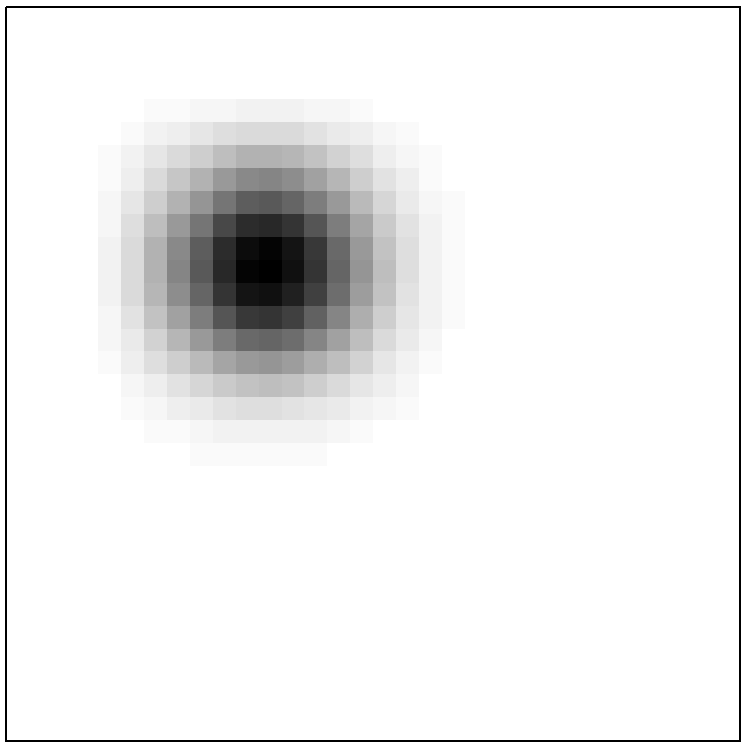
\includegraphics[width=2.5cm]{images/bump_betaold/bump_beta1_09}&
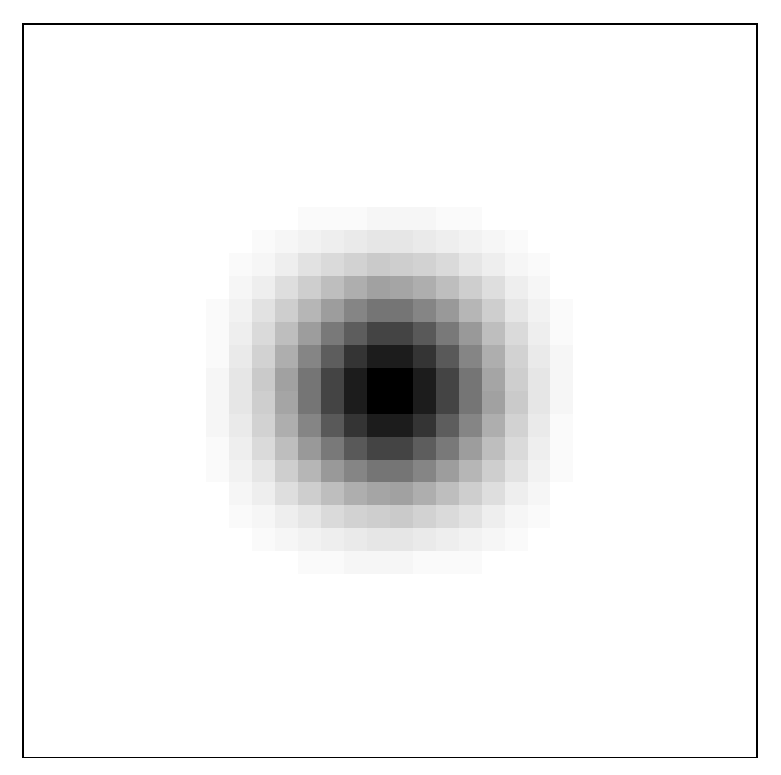
\includegraphics[width=2.5cm]{images/bump_betaold/bump_beta1_17}&
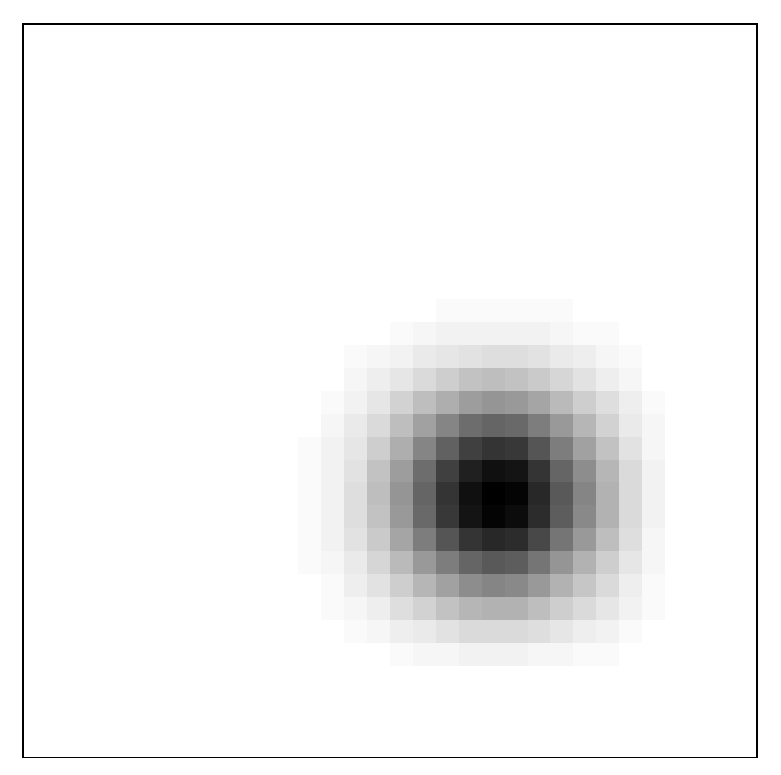
\includegraphics[width=2.5cm]{images/bump_betaold/bump_beta1_25}&

\includegraphics[width=2.5cm]{images/bump_betaold/bump_beta1_33}\\
$t=0$&$t=1/4$&$t=1/2$&$t=3/4$&$t=1$ % \vspace{-0.1cm}
\end{tabular}
\caption{\label{fig:data_bump} 
Display of $f^\star(\cdot,t)$ for several value of $t$ (note that for $t=0$ and $t=1$, this corresponds to $f^0$ and $f^1$). The grayscale values are linearly interpolating from black to white between 0 and the maximum value of $f^\star$. 
% \vspace{-0.2cm}% 10^{-8} 0.017
}
\end{center}
\end{figure}

For each algorithm, we perform an exhaustive search of the best possible set of parameters. These optimal parameters are those minimizing $\norm{(m^\star,f^\star) - (\iter{m},\iter{f})}$, the $\ell^2$ distance between $f^\star$ and the output of the algorithm after $\ell=100$ iterations. The obtained  parameters for this data set are:  $\ga=1/350$ for ADMM on the dual, $(\ga=1/240,\al=1.983)$ for DR and $\si=85$ for PD. For PD, we found that simply setting $\tau=\frac{0.99}{\si \norm{\interp}^2}$ leads to almost optimal convergence rate in our tests, so we use this rule to only introduce a single parameter $\si$. Note that this parameter choice is within the range of parameters $\sigma \tau \norm{\interp}^2<1$ that guaranties convergence of the PD method. Figure~\ref{fig:comp_bump} displays, for this optimal choice of parameters, the evolution of the cost function value as well as the  convergence toward $(m^\star,f^\star)$ as a function of the iteration number $\ell$. 

One can observe that the quality of the estimation can not be deduced from the cost function evolution since the functional is very flat. Indeed, an almost minimal value of the function minimum is reached by all the algorithms after roughly $10^3$ iterations, whereas the $\ell^2$ distance to the reference solution continue to decrease almost linearly in log-log scale.

\begin{figure}[!ht]
\begin{center}
\begin{tabular}{ccc}
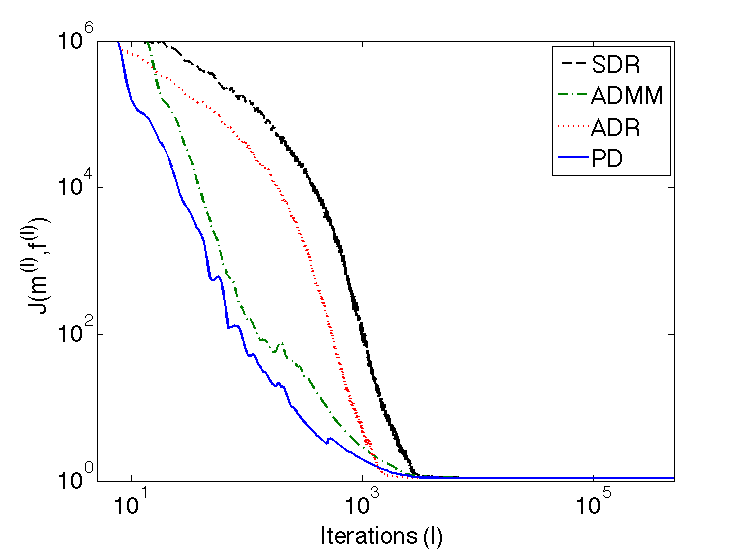
\includegraphics[trim=30 10 40 20,clip,width=0.33\textwidth]{images/J}&\hspace{-0.5cm}
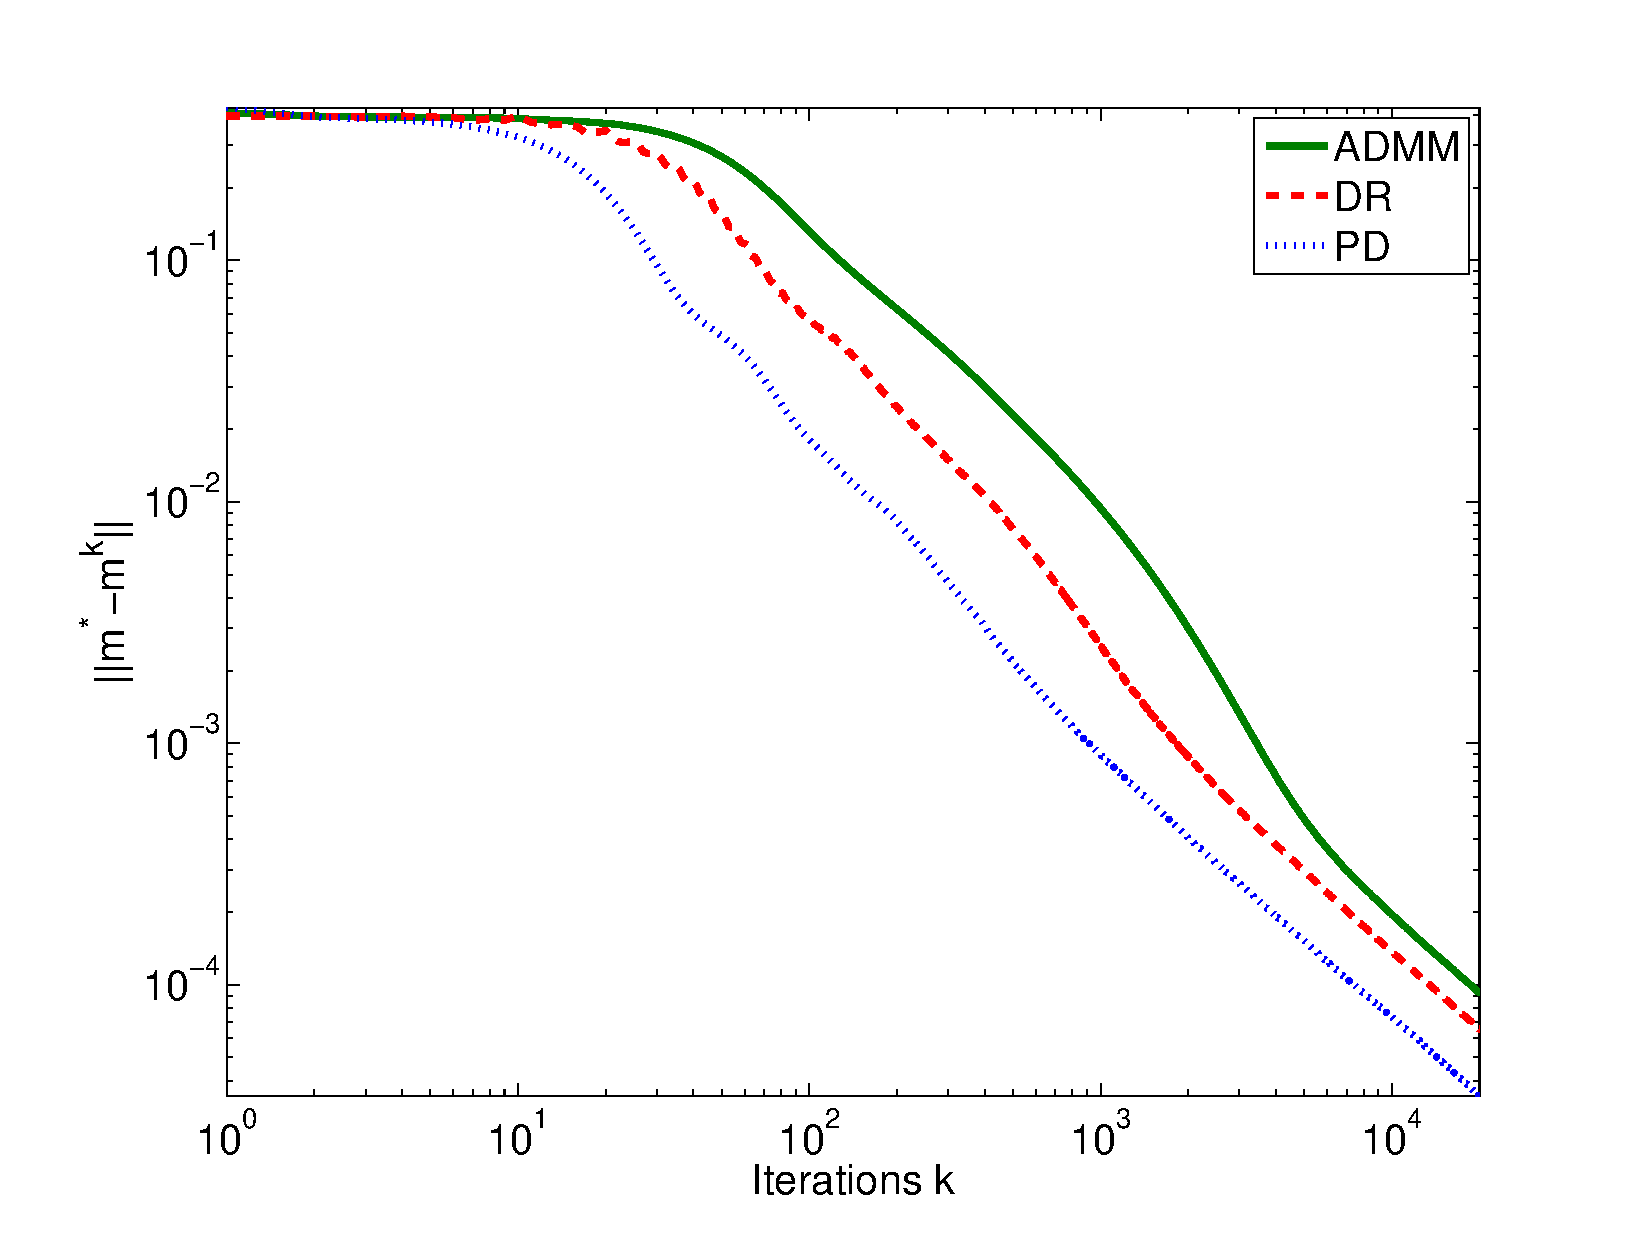
\includegraphics[trim=30 10 40 20,clip,width=0.33\textwidth]{images/convergence_m}&\hspace{-0.5cm}
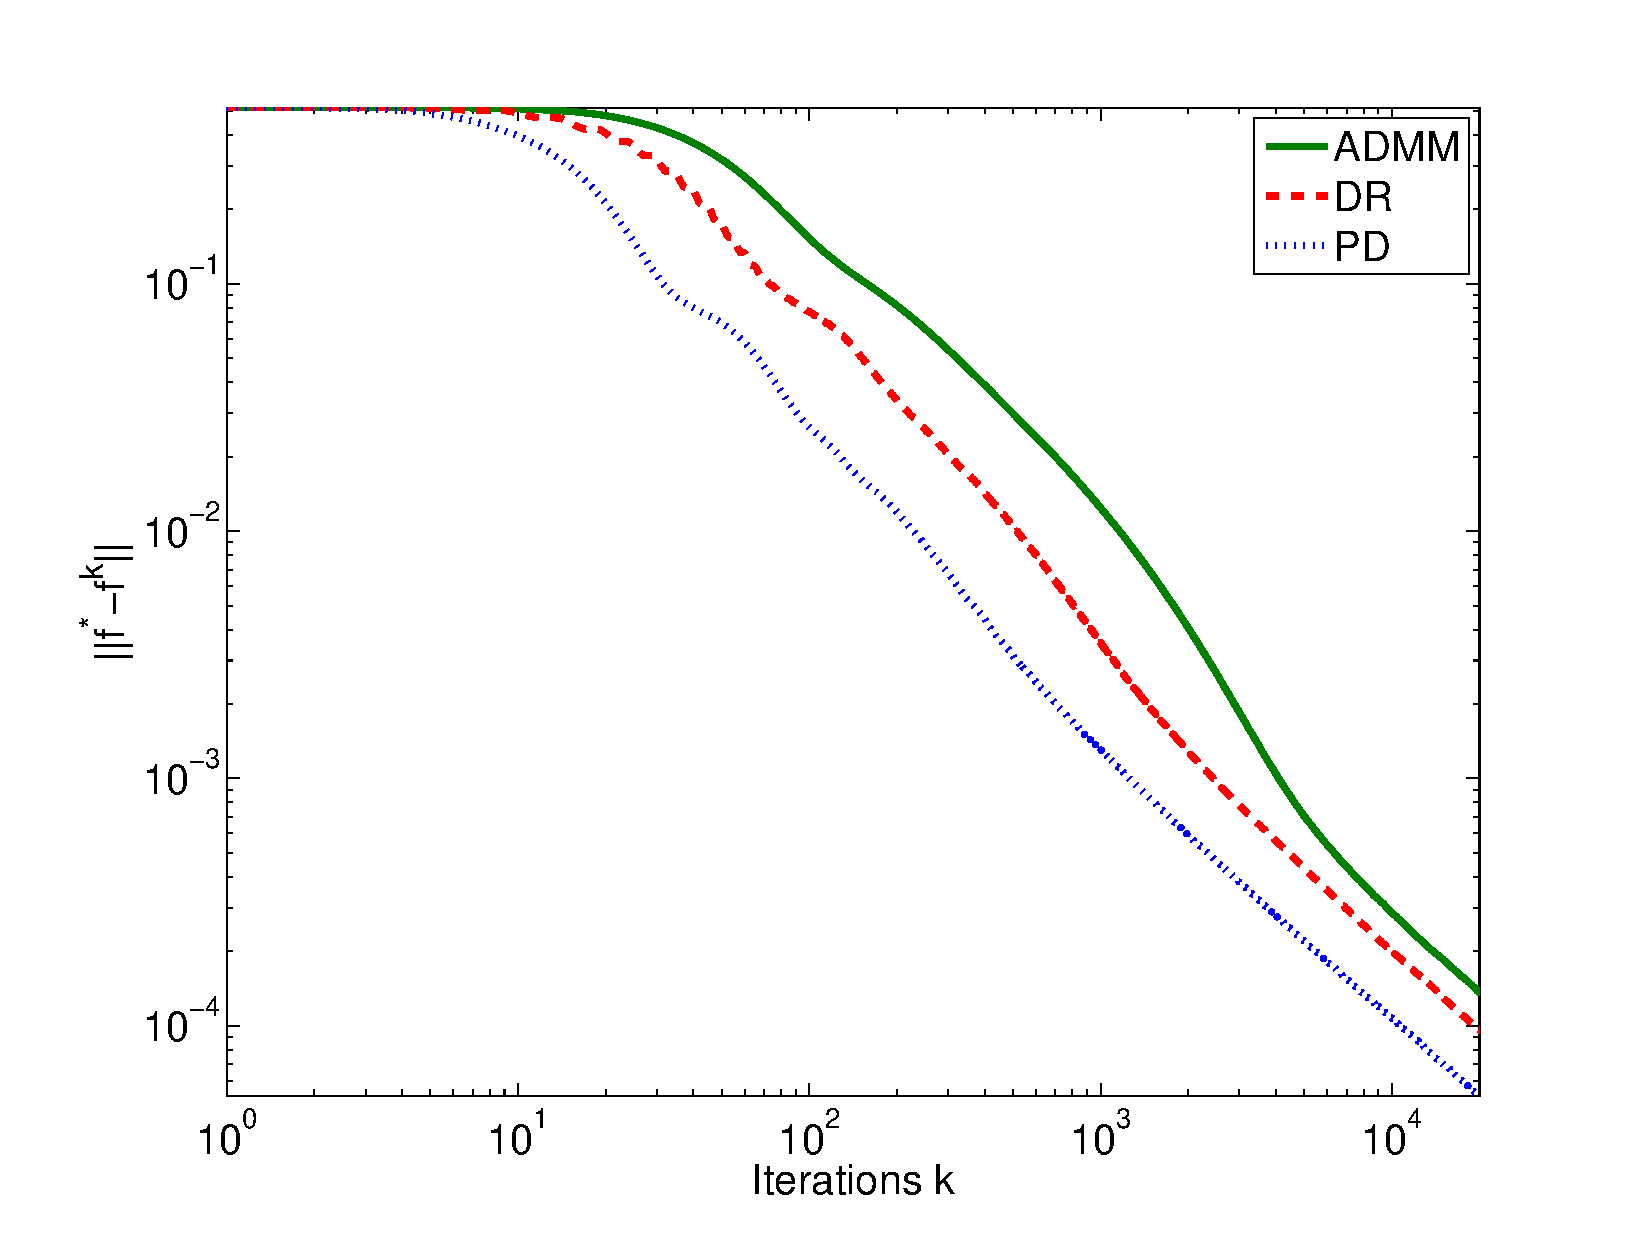
\includegraphics[trim=30 10 40 20,clip,width=0.33\textwidth]{images/convergence_f}\vspace{0.1cm}\\
$\Jfunc( \iter{m}, \iter{f} )$&\hspace{-0.5cm}$ \norm{m^\star-\iter{m}}$ &\hspace{-0.5cm}$ \norm{f^\star-\iter{f}}$ \vspace{-0.2cm}
\end{tabular}
\caption{\label{fig:comp_bump} 
	At each iteration $\ell$, we plot the value of the cost function $\Jfunc$ and the distance between the reference solution $(m^\star,f^\star)$ and the estimation $(\iter{m},\iter{f})$ for the different proximal splitting algorithms with the best found parameters. }
\end{center}
\end{figure}

When comparing the three approaches, PD presents the fastest convergence rate to the reference solution and the relaxed DR algorithm performs better than ADDM on the dual, which shows the advantage of introducing the $\al$ parameter. Note also that the computational cost is smaller for PD, as it takes\footnote{For our Matlab implementation on a standard laptop computer.} $0.13$s for one PD iteration and $0.2s$ for one DR or ADMM iteration for this example. 

% It can also  be noticed that PD is easier to parameterize. Indeed,  from the necessary relation $\sigma \tau \norm{\interp}^2<1$, one can chose $\si$ and then automatically fix $\tau=\frac{0.99}{\si \norm{\interp}^2}$. The exhaustive search has been realized in this way, thus involving a limited set of possible parameters for PD.




%%%%%%%%%%%%%%%%%%%%%%%%%%%%%%%%%%%%%%%%%%%%%%%%%%%%%%%%%%%%%%%%
%%%%%%%%%%%%%%%%%%%%%%%%%%%%%%%%%%%%%%%%%%%%%%%%%%%%%%%%%%%%%%%%
%%%%%%%%%%%%%%%%%%%%%%%%%%%%%%%%%%%%%%%%%%%%%%%%%%%%%%%%%%%%%%%%
\subsection{Interpolation Between $L^2$-Wasserstein and $H^{-1}$}

% Gabriel :  Wich $\ell$ is used ?

We first apply the PD algorithm for different values of $\beta$ on the bump example introduced in the previous section. The results are presented in the Figure~\ref{fig:generalized_bump}, which shows the level-lines of the estimated densities $\iter{f}(\cdot,t)$ for $\ell=1000$ iterations. It shows the evolution of the solution between a $H^{-1}$ linear interpolation ($\beta=0$) and a displacement interpolation with transport ($\beta=1$). 

% Gabriel : Ceci n'est pas terrible !! Essayer de le corriger ?
% Nicolas: Corrig�

% Notice that the minimum value of $f^0$ and $f^1$ has been bounded with the value $10^{-8}$, so that the true transport is not exactly a translation for the case $\beta=1$. This explains the slight deformations of the circles in the last line of Figure \ref{fig:generalized_bump}. 


\newcommand{\sidecap}[1]{ {\begin{sideways}\parbox{1.6cm}{\centering #1}\end{sideways}} }
\begin{figure}[!ht]
\begin{center}
\begin{tabular}{cccccccccc}
\sidecap{$\beta=0$ } &\hspace{-0.45cm}
%\animategraphics[palindrome=true,width=1.6cm]{6}{images/bump_anim/bump_beta_0_iso_}{01}{33}&
%\movie[mouse=true,palindrome=true]{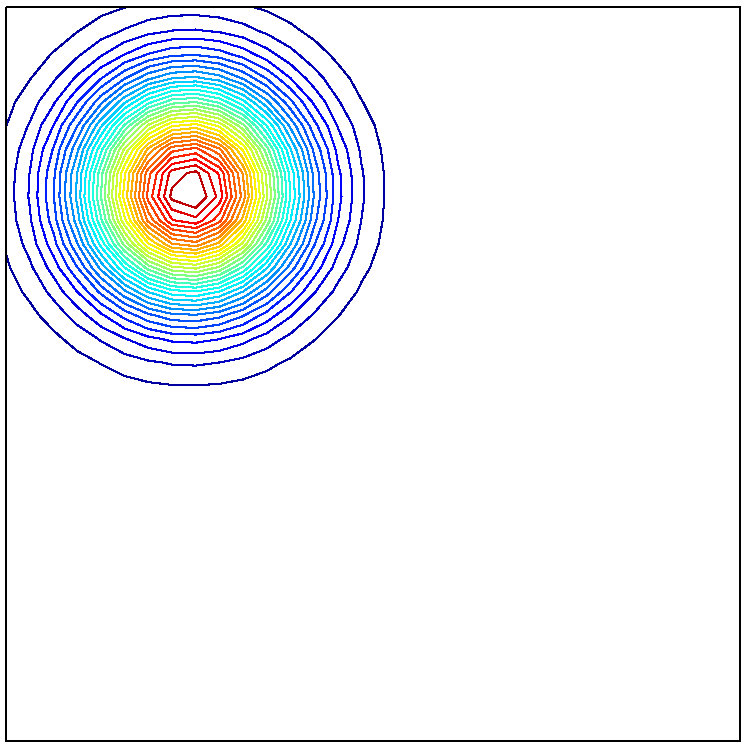
\includegraphics[width=1.6cm]{images/bump_beta/bump_beta_0_iso_01}}{images/bump_beta/beta_0.avi}&
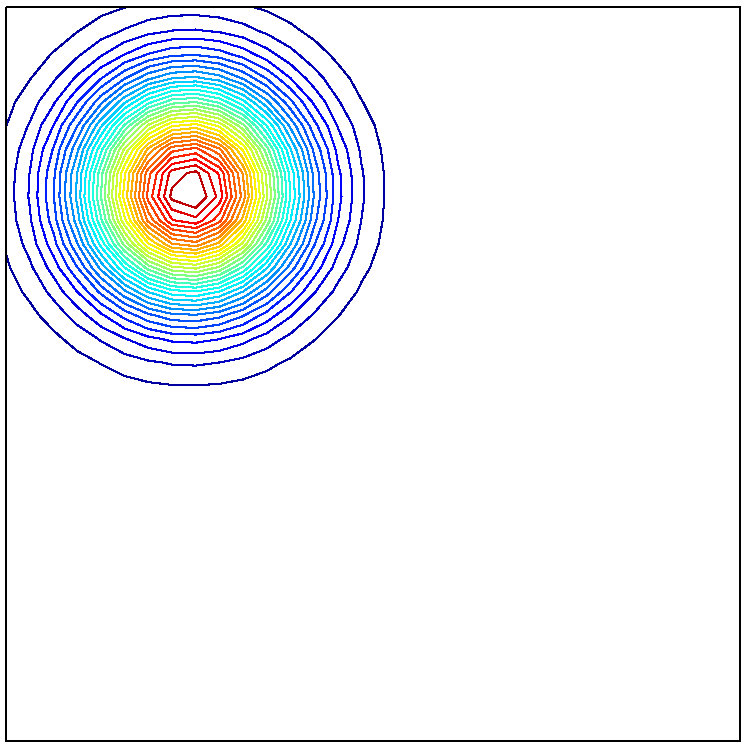
\includegraphics[width=1.6cm]{images/bump_beta/bump_beta_0_iso_01}&
\hspace{-0.45cm}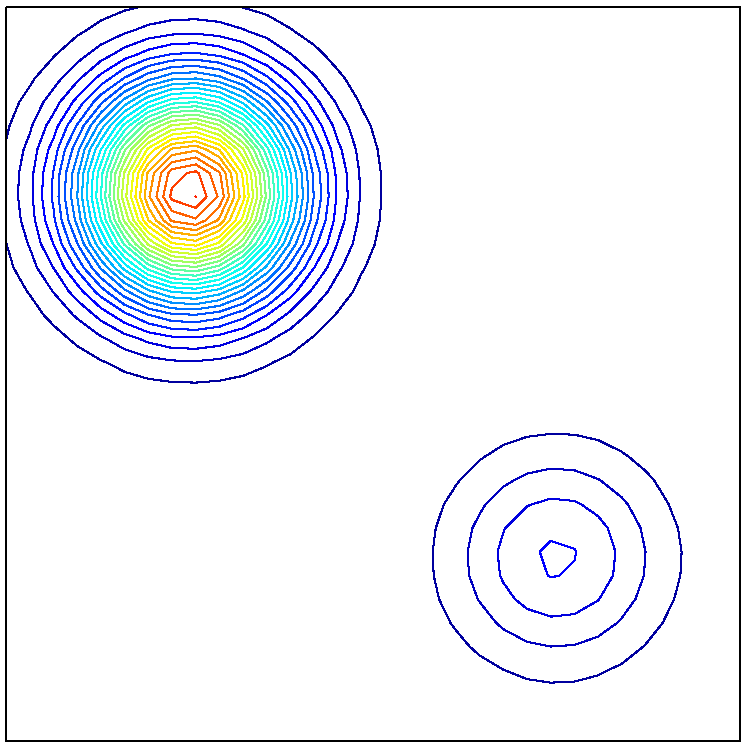
\includegraphics[width=1.6cm]{images/bump_beta/bump_beta_0_iso_05}&
\hspace{-0.45cm}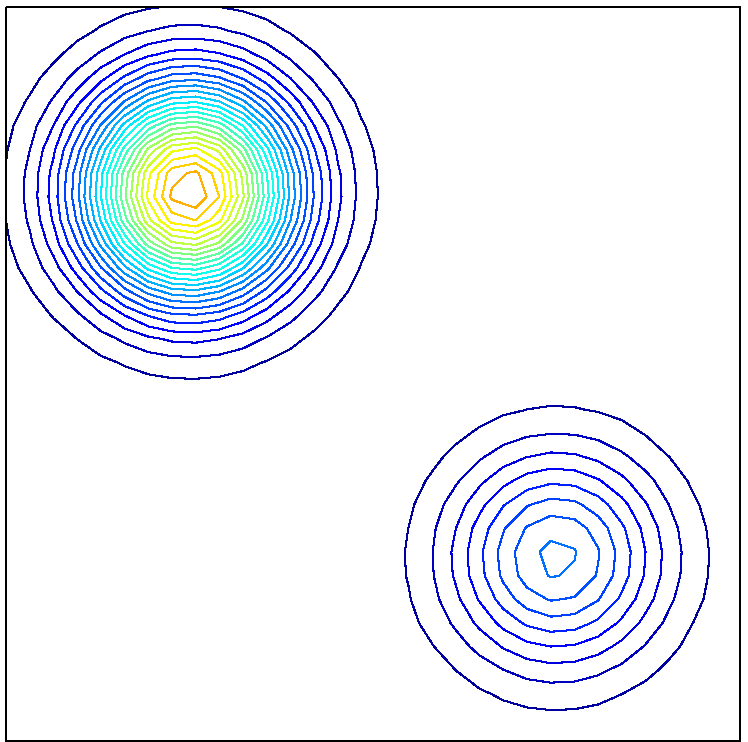
\includegraphics[width=1.6cm]{images/bump_beta/bump_beta_0_iso_09}&
\hspace{-0.45cm}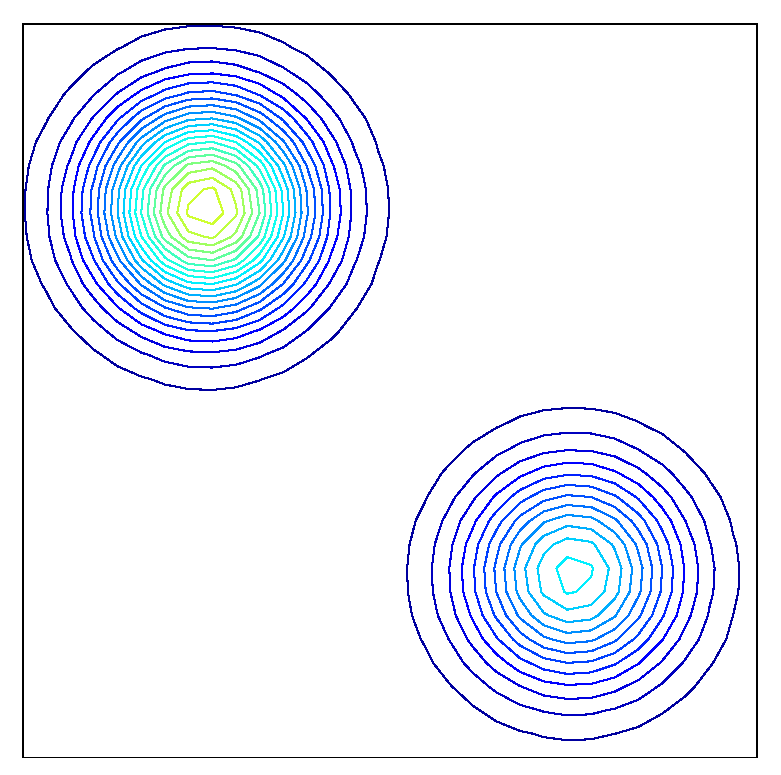
\includegraphics[width=1.6cm]{images/bump_beta/bump_beta_0_iso_13}&
\hspace{-0.45cm}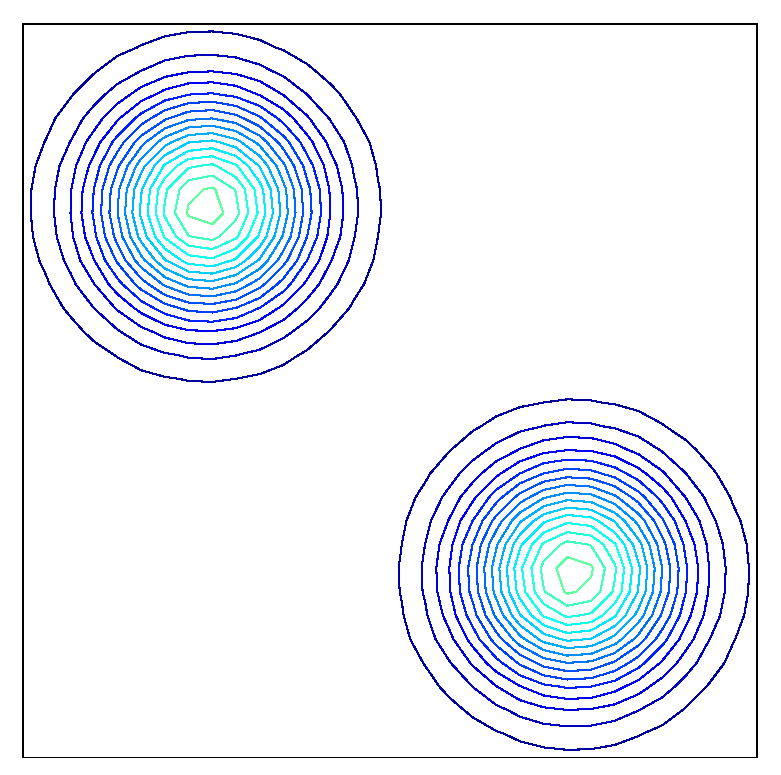
\includegraphics[width=1.6cm]{images/bump_beta/bump_beta_0_iso_17}&
\hspace{-0.45cm}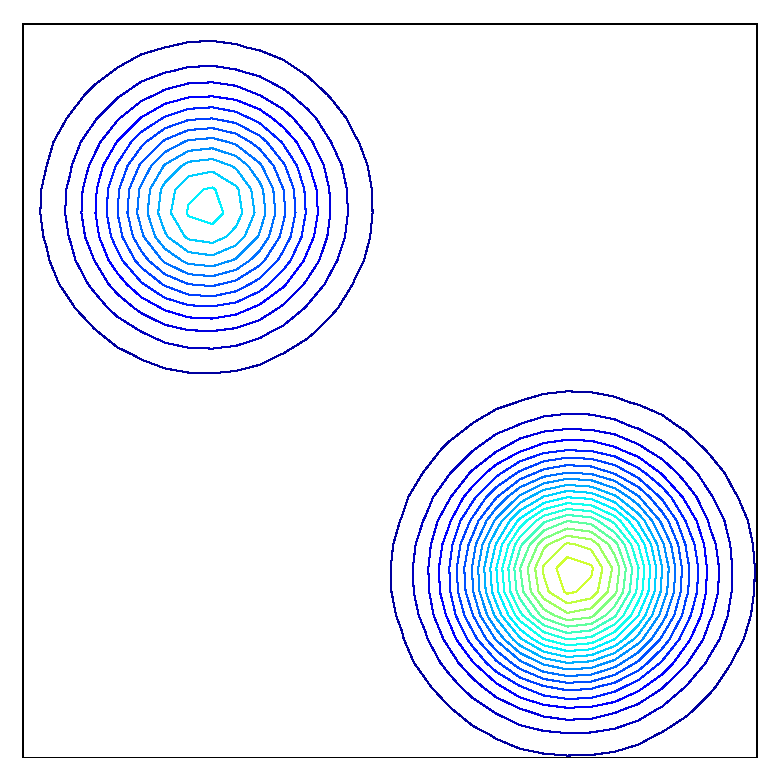
\includegraphics[width=1.6cm]{images/bump_beta/bump_beta_0_iso_21}&
\hspace{-0.45cm}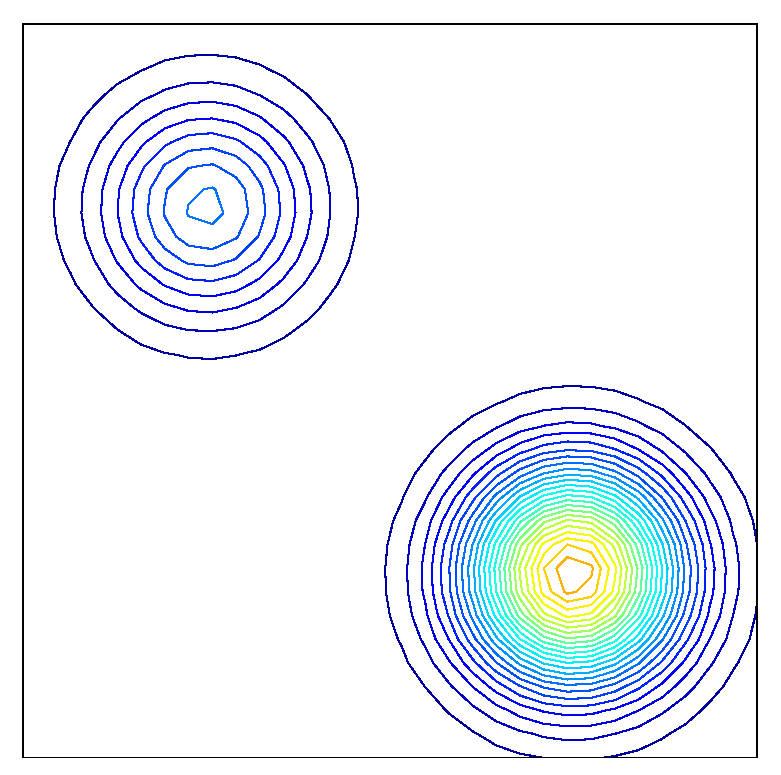
\includegraphics[width=1.6cm]{images/bump_beta/bump_beta_0_iso_25}&
\hspace{-0.45cm}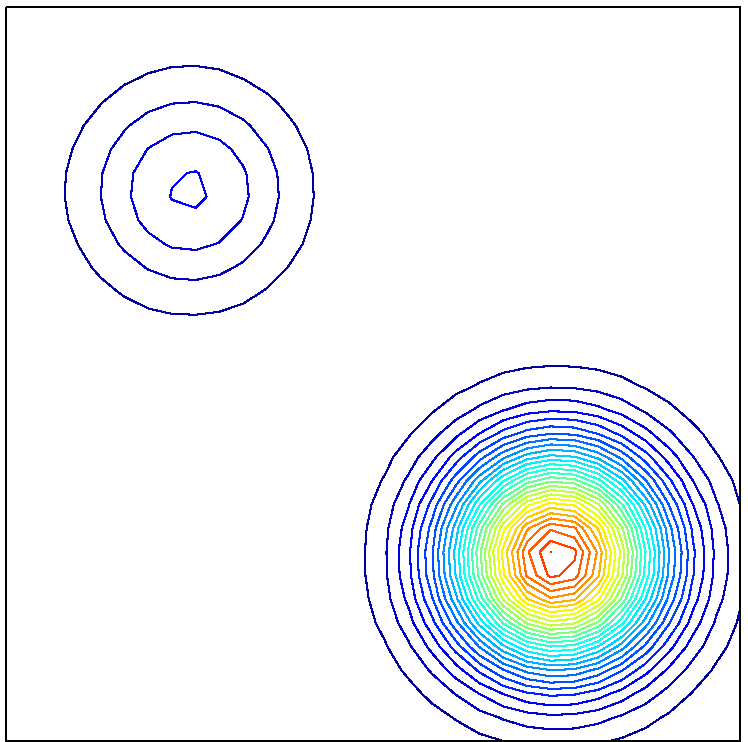
\includegraphics[width=1.6cm]{images/bump_beta/bump_beta_0_iso_29}&
\hspace{-0.45cm}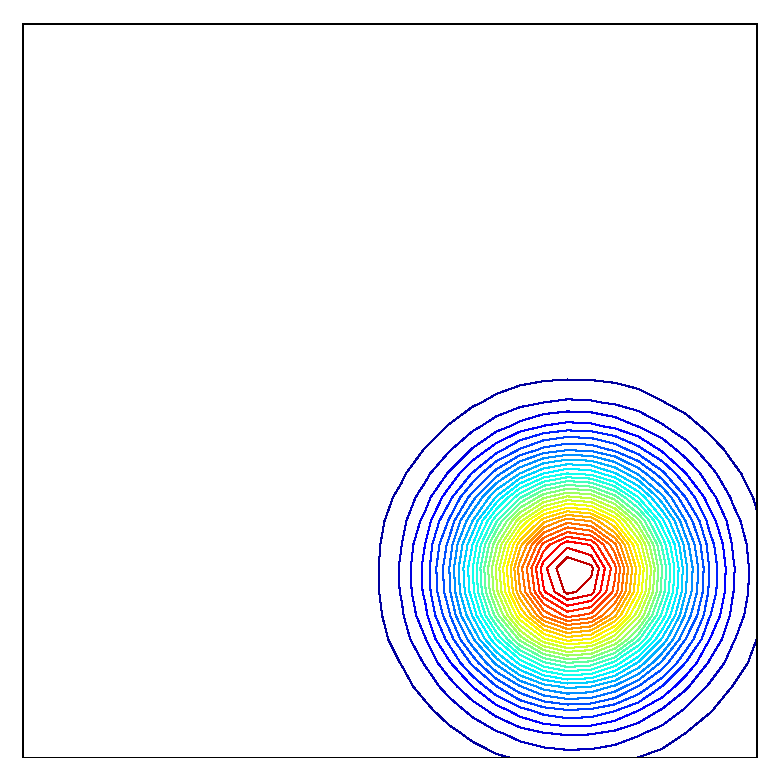
\includegraphics[width=1.6cm]{images/bump_beta/bump_beta_0_iso_33}\\
\sidecap{$\beta=1/4$ } &\hspace{-0.45cm}
%\animategraphics[palindrome=true,width=1.6cm]{6}{images/bump_anim/bump_beta_25_iso_}{01}{33}&
%\movie[mouse=true,palindrome=true]{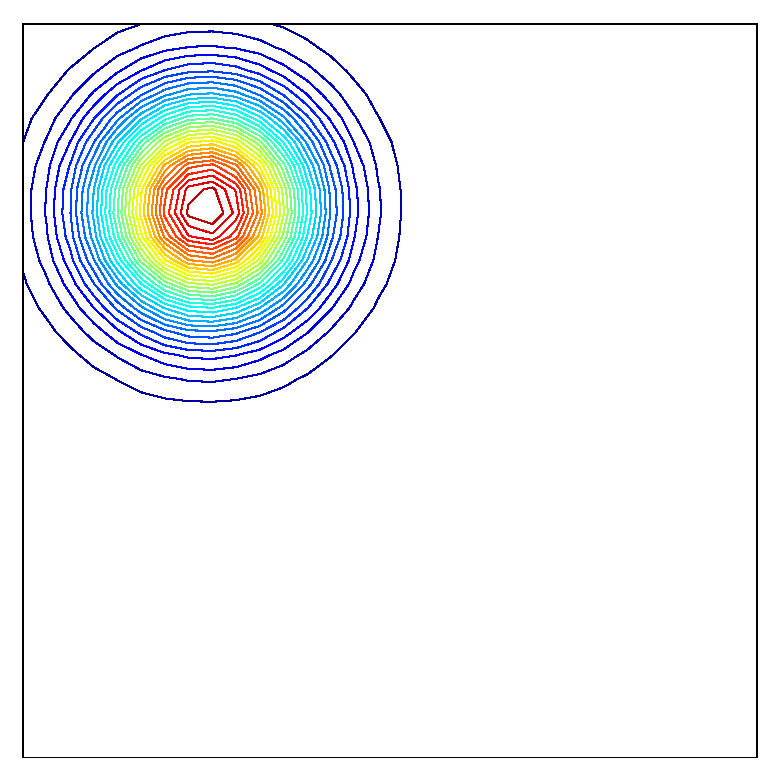
\includegraphics[width=1.6cm]{images/bump_beta/bump_beta_25_iso_01}}{images/bump_beta/beta_25.avi}&
%
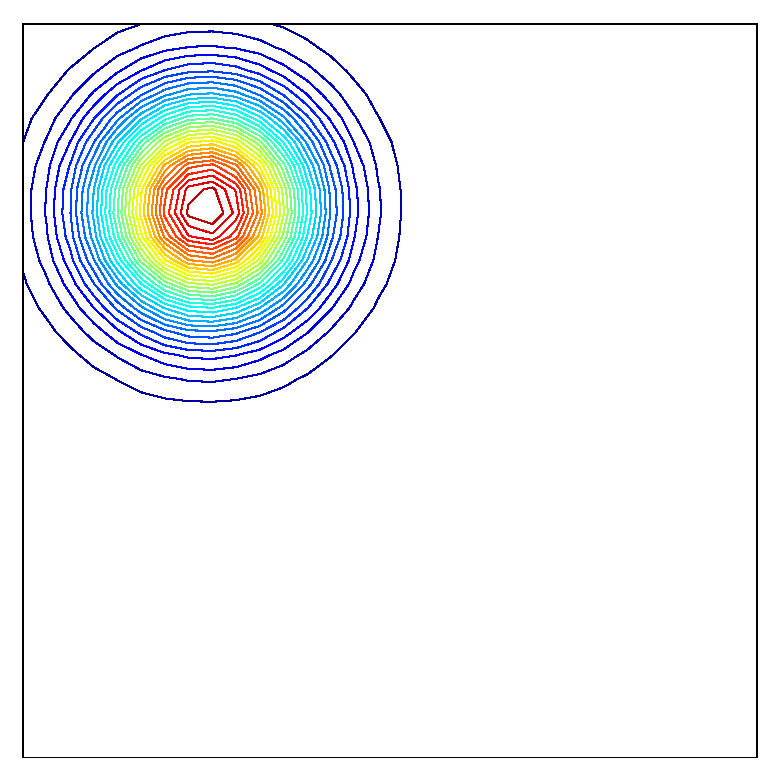
\includegraphics[width=1.6cm]{images/bump_beta/bump_beta_25_iso_01}&
\hspace{-0.45cm}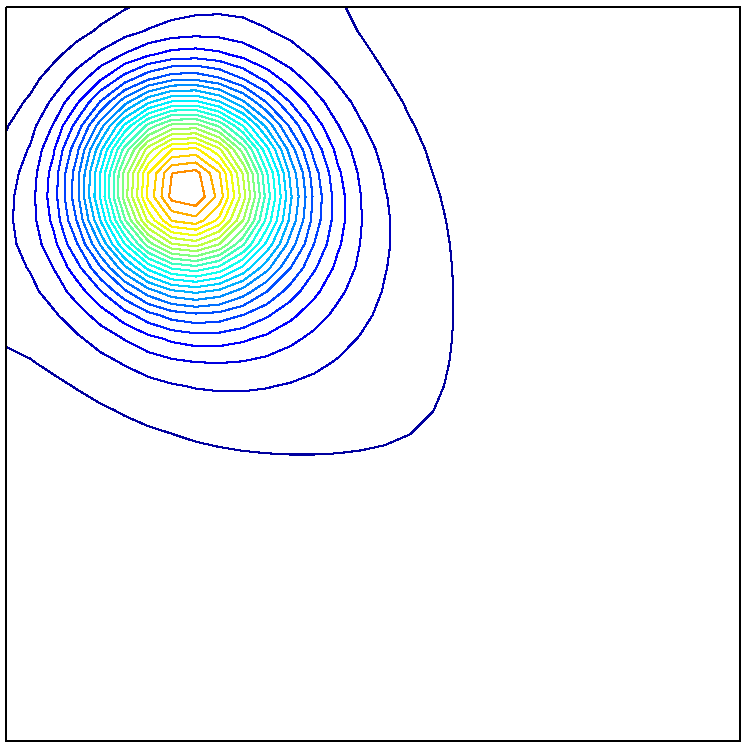
\includegraphics[width=1.6cm]{images/bump_beta/bump_beta_25_iso_05}&
\hspace{-0.45cm}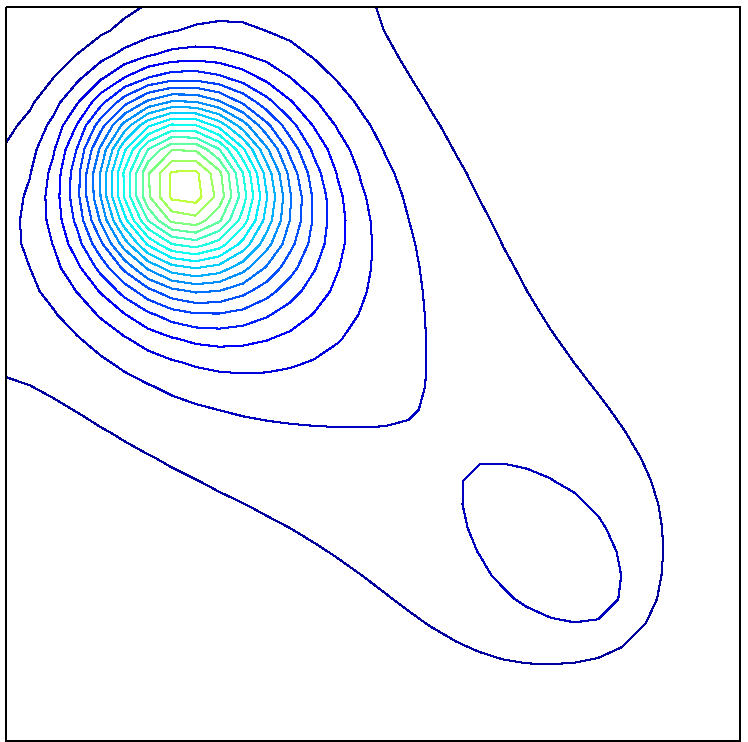
\includegraphics[width=1.6cm]{images/bump_beta/bump_beta_25_iso_09}&
\hspace{-0.45cm}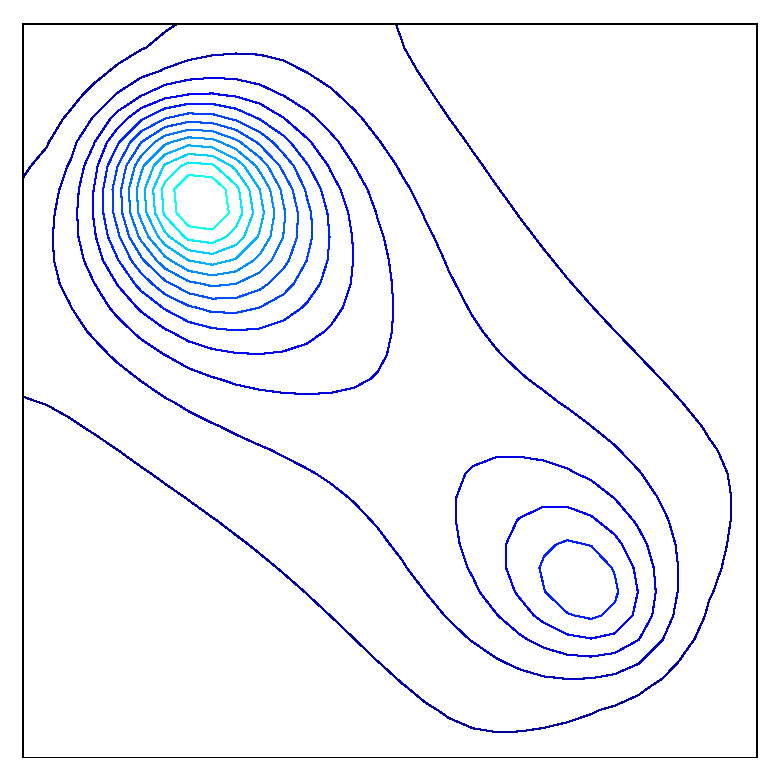
\includegraphics[width=1.6cm]{images/bump_beta/bump_beta_25_iso_13}&
\hspace{-0.45cm}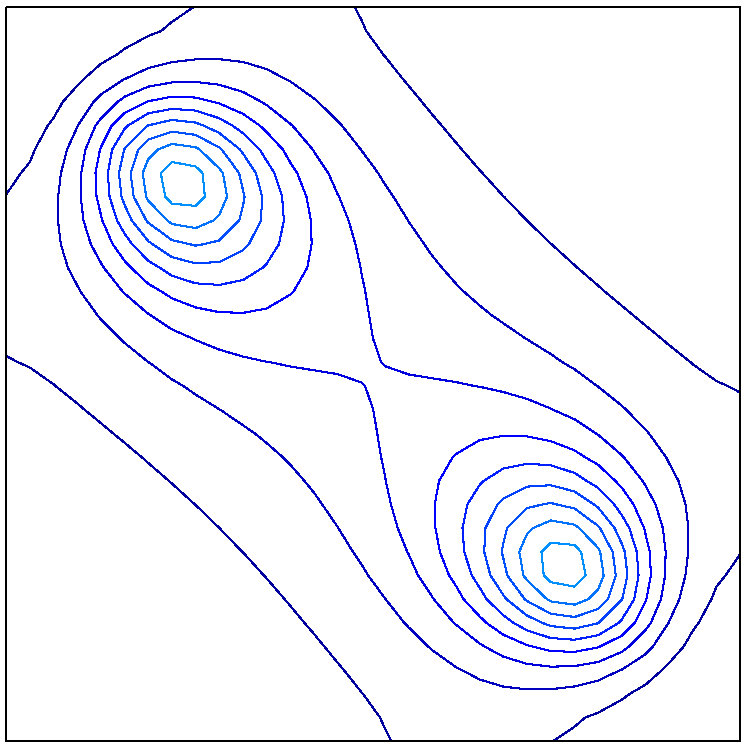
\includegraphics[width=1.6cm]{images/bump_beta/bump_beta_25_iso_17}&
\hspace{-0.45cm}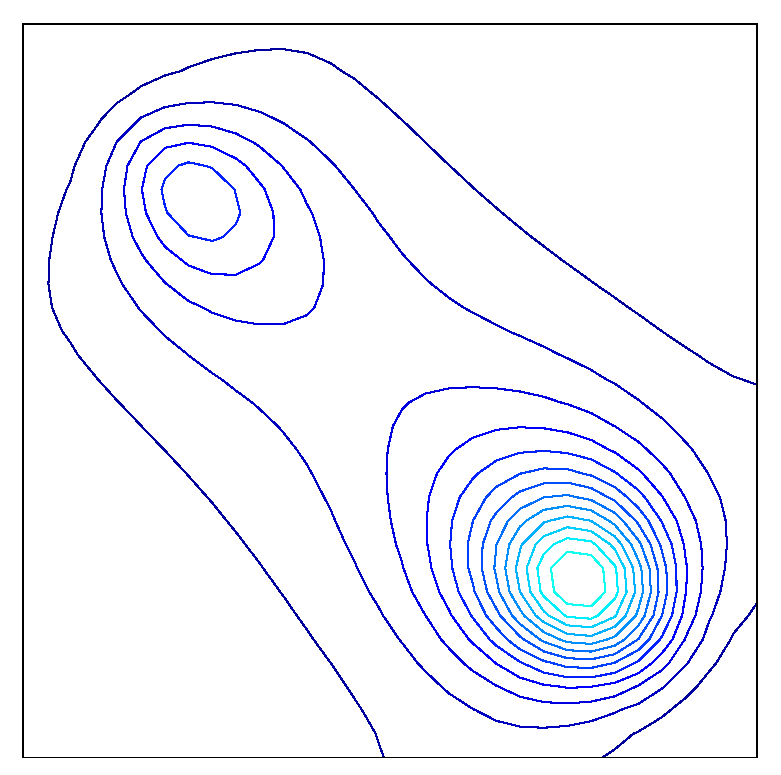
\includegraphics[width=1.6cm]{images/bump_beta/bump_beta_25_iso_21}&
\hspace{-0.45cm}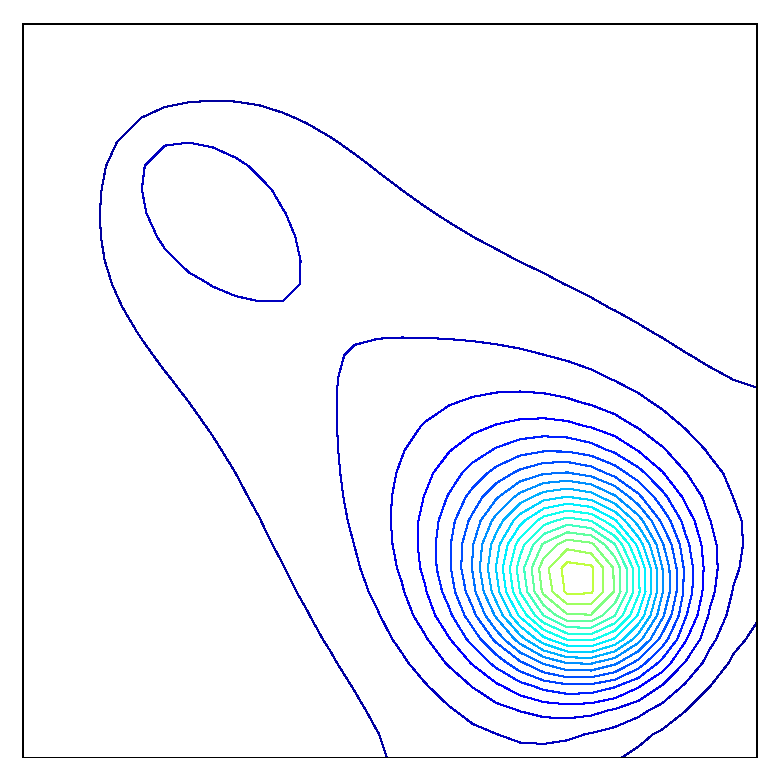
\includegraphics[width=1.6cm]{images/bump_beta/bump_beta_25_iso_25}&
\hspace{-0.45cm}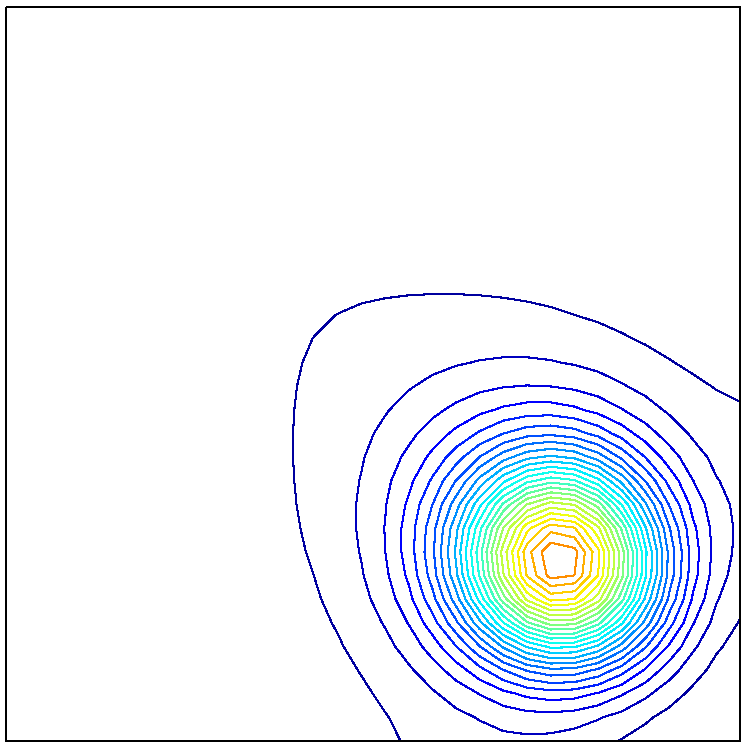
\includegraphics[width=1.6cm]{images/bump_beta/bump_beta_25_iso_29}&
\hspace{-0.45cm}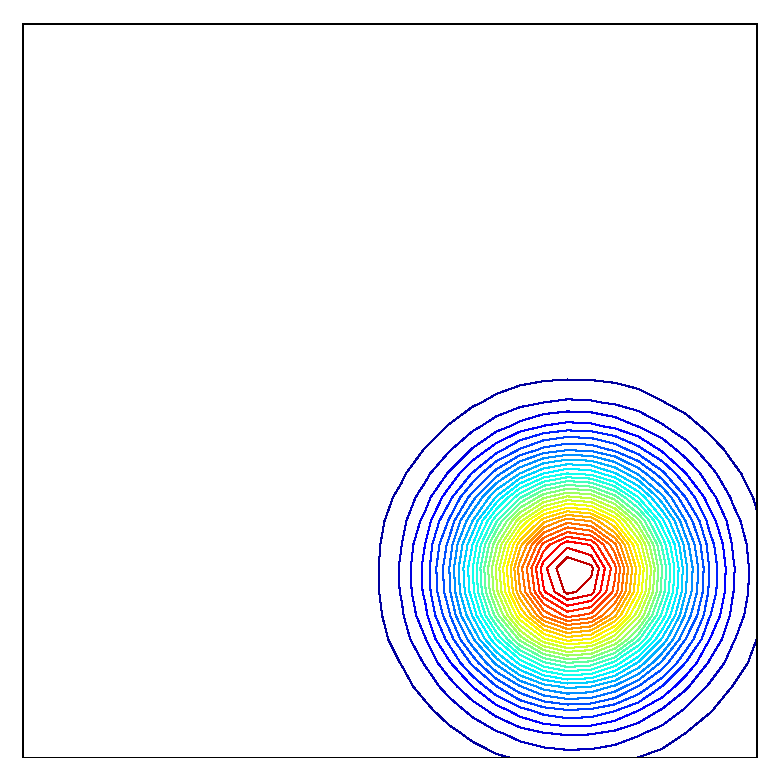
\includegraphics[width=1.6cm]{images/bump_beta/bump_beta_25_iso_33}\\
\sidecap{$\beta=1/2$ } &\hspace{-0.45cm}
%\animategraphics[palindrome=true,width=1.6cm]{6}{images/bump_anim/bump_beta_05_iso_}{01}{33}&
%\movie[mouse=true,palindrome=true]{\includegraphics[width=1.6cm]{images/bump_beta/bump_beta_05_iso_01}}{images/bump_beta/beta_05.avi}&
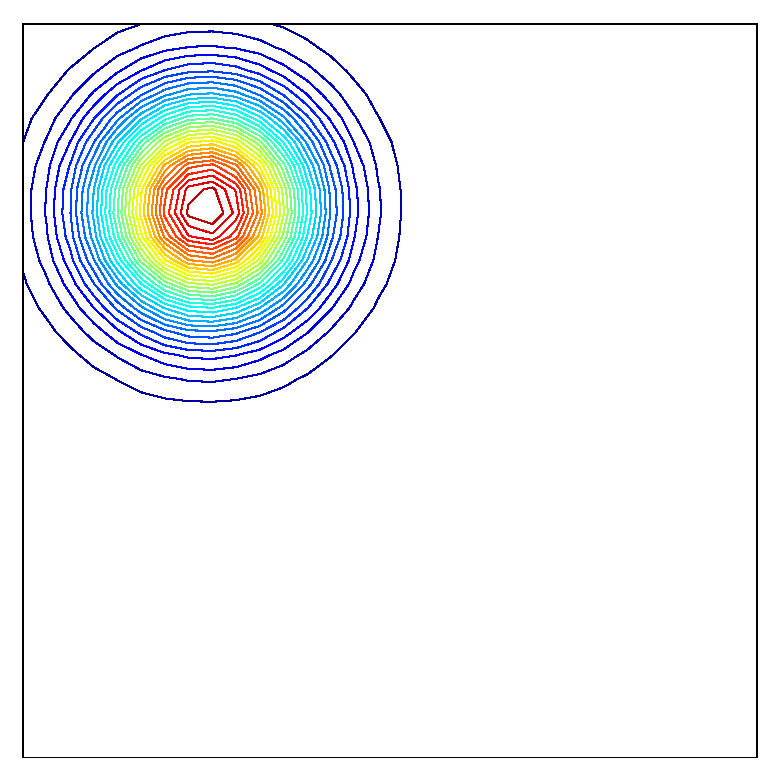
\includegraphics[width=1.6cm]{images/bump_beta/bump_beta_50_iso_01}&
\hspace{-0.45cm}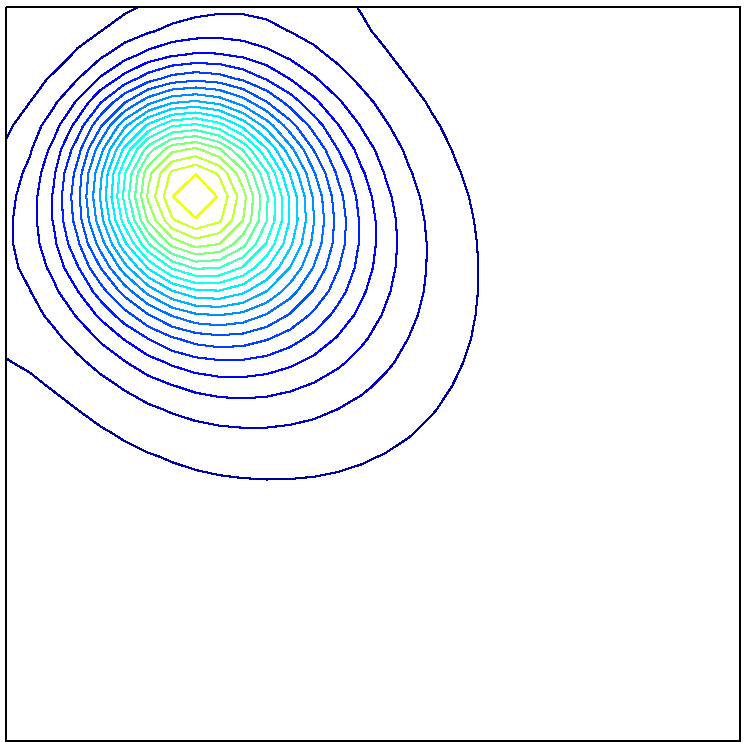
\includegraphics[width=1.6cm]{images/bump_beta/bump_beta_50_iso_05}&
\hspace{-0.45cm}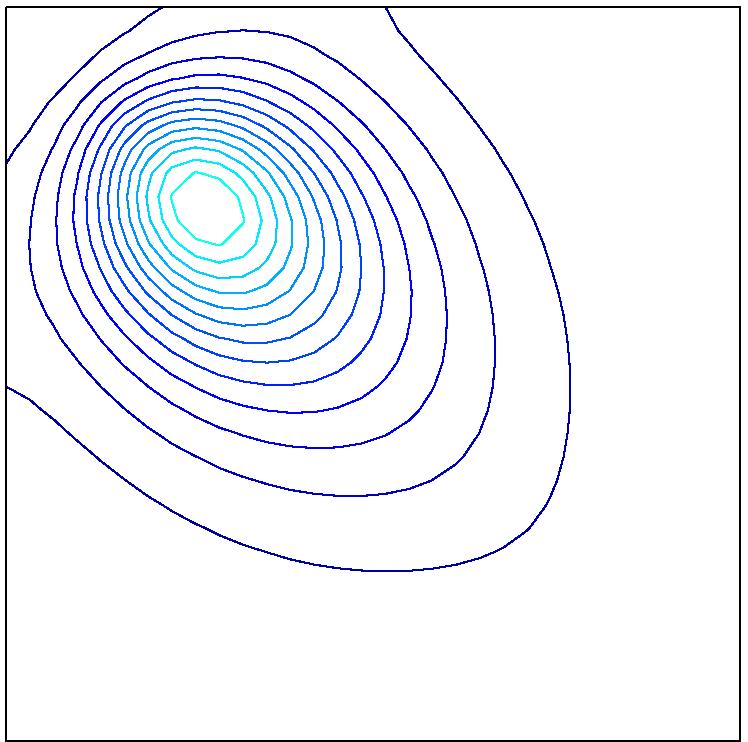
\includegraphics[width=1.6cm]{images/bump_beta/bump_beta_50_iso_09}&
\hspace{-0.45cm}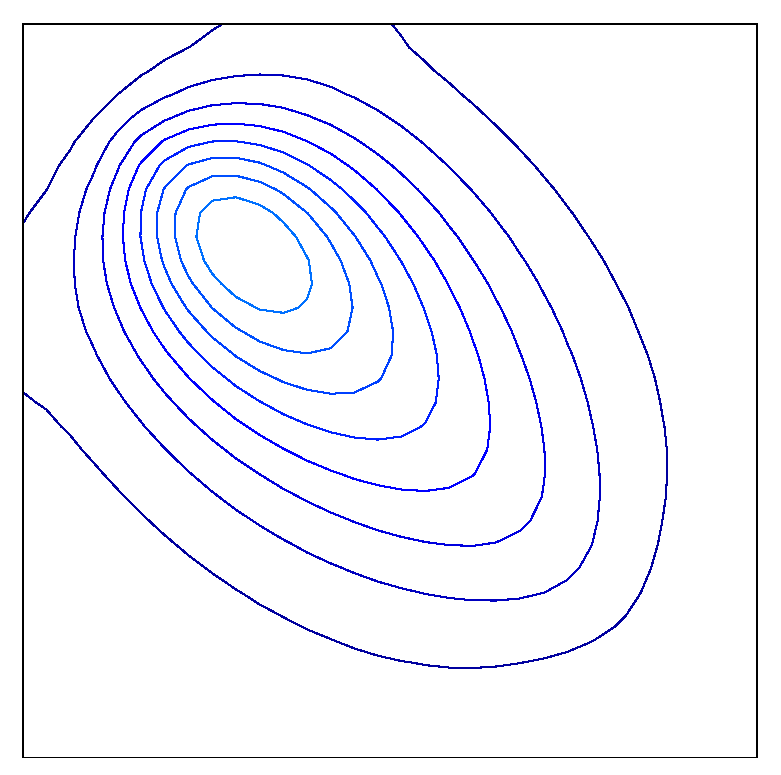
\includegraphics[width=1.6cm]{images/bump_beta/bump_beta_50_iso_13}&
\hspace{-0.45cm}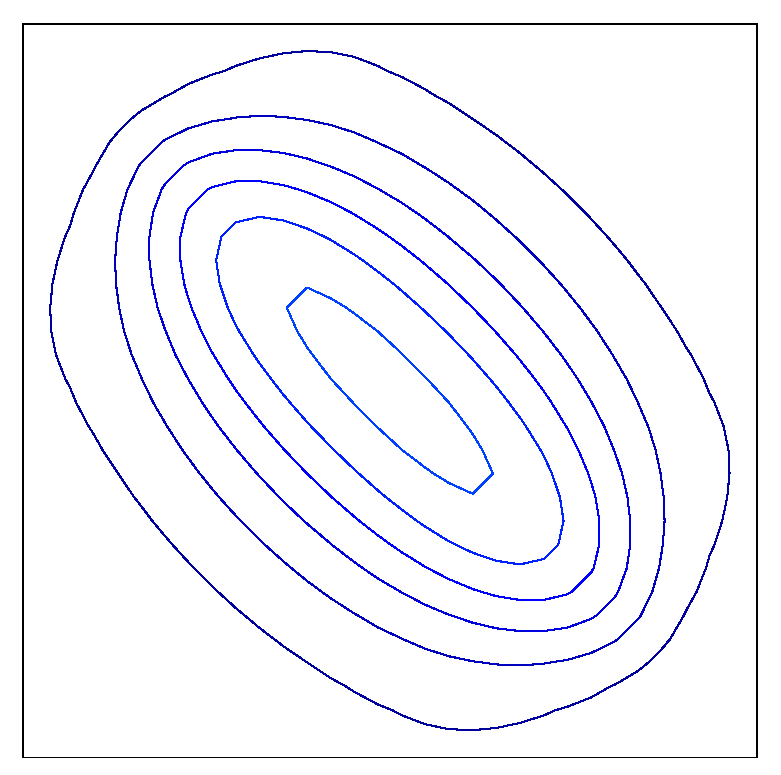
\includegraphics[width=1.6cm]{images/bump_beta/bump_beta_50_iso_17}&
\hspace{-0.45cm}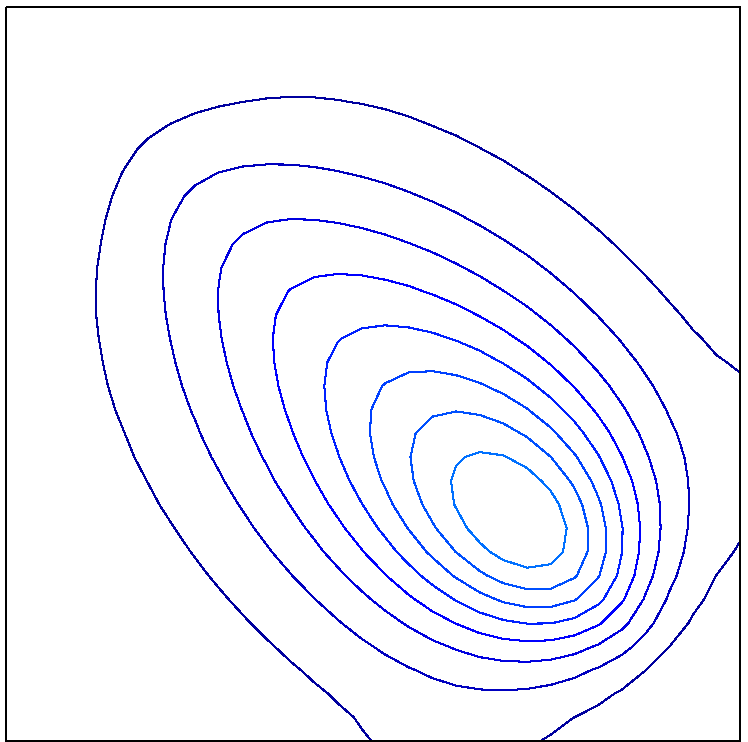
\includegraphics[width=1.6cm]{images/bump_beta/bump_beta_50_iso_21}&
\hspace{-0.45cm}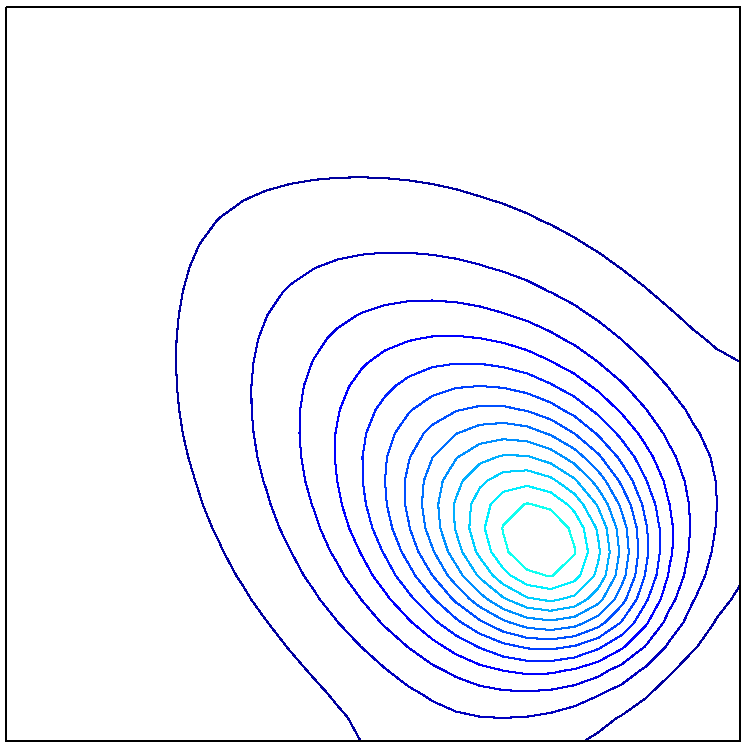
\includegraphics[width=1.6cm]{images/bump_beta/bump_beta_50_iso_25}&
\hspace{-0.45cm}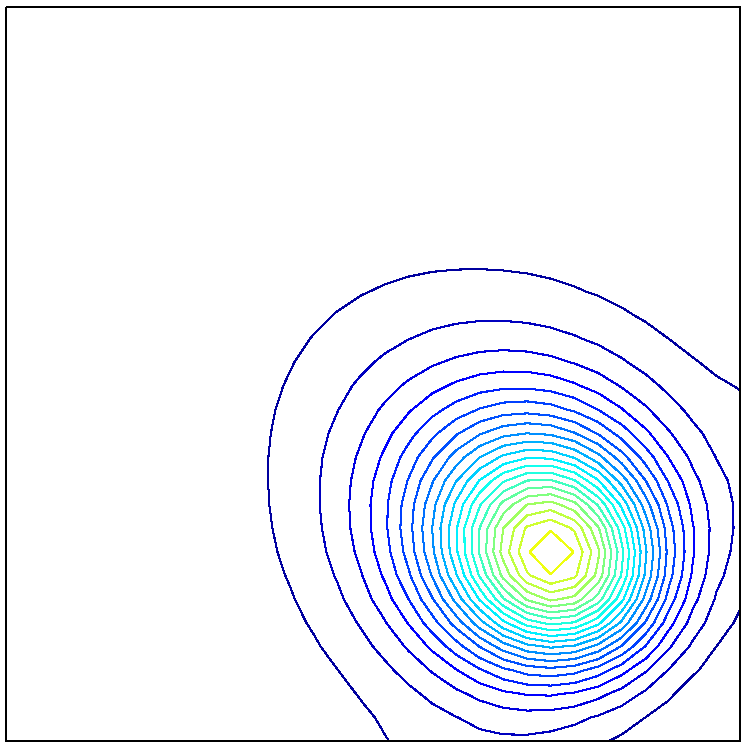
\includegraphics[width=1.6cm]{images/bump_beta/bump_beta_50_iso_29}&
\hspace{-0.45cm}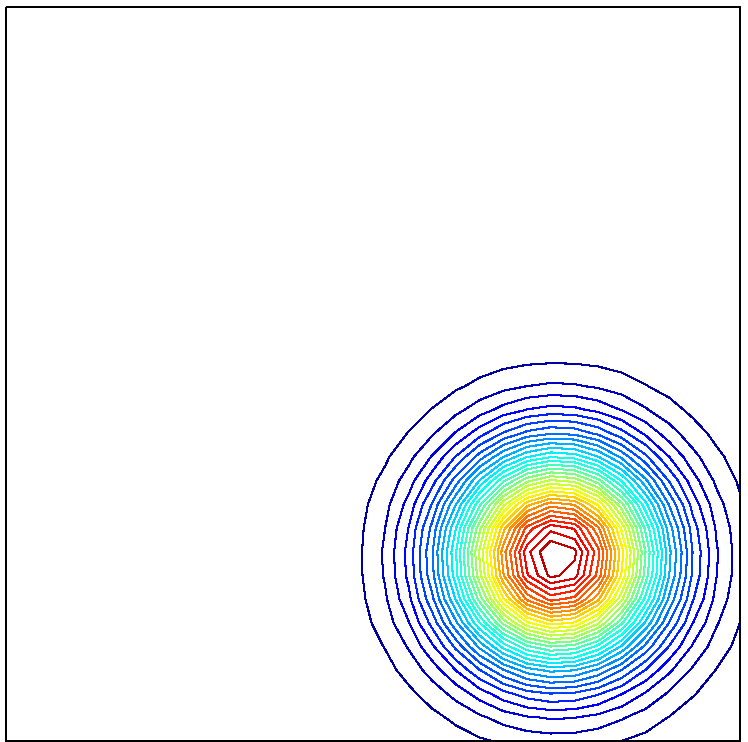
\includegraphics[width=1.6cm]{images/bump_beta/bump_beta_50_iso_33}\\
\sidecap{$\beta=3/4$ } &\hspace{-0.45cm}
%\animategraphics[palindrome=true,width=1.6cm]{6}{images/bump_anim/bump_beta_75_iso_}{01}{33}&
%\movie[mouse=true,palindrome=true]{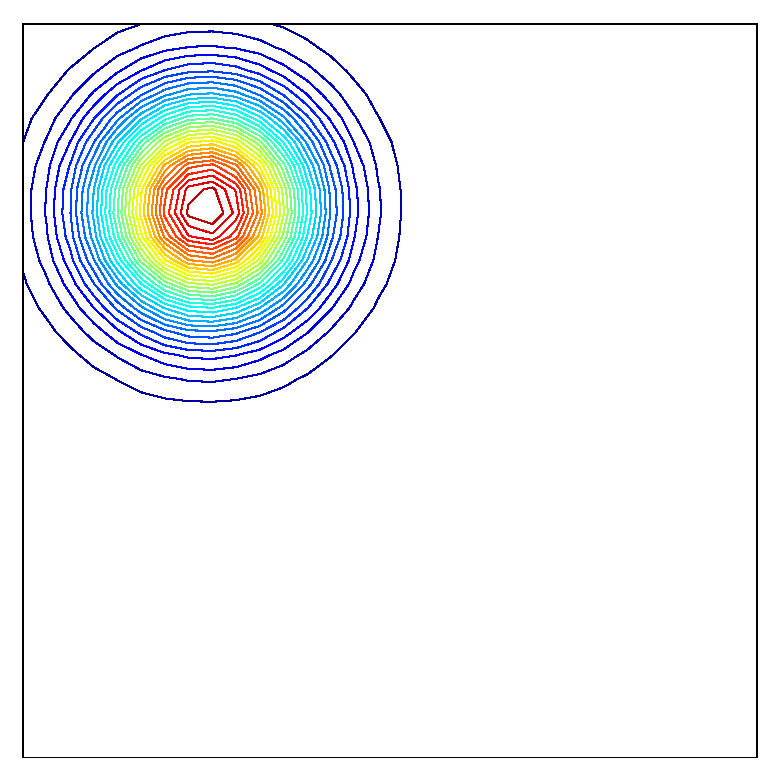
\includegraphics[width=1.6cm]{images/bump_beta/bump_beta_75_iso_01}}{images/bump_beta/beta_75.avi}&
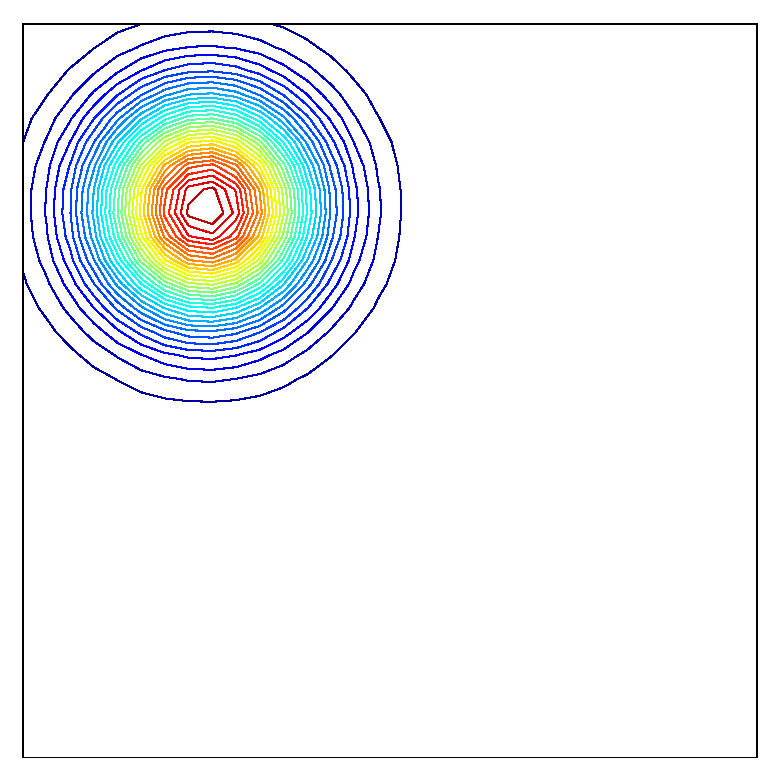
\includegraphics[width=1.6cm]{images/bump_beta/bump_beta_75_iso_01}&
\hspace{-0.45cm}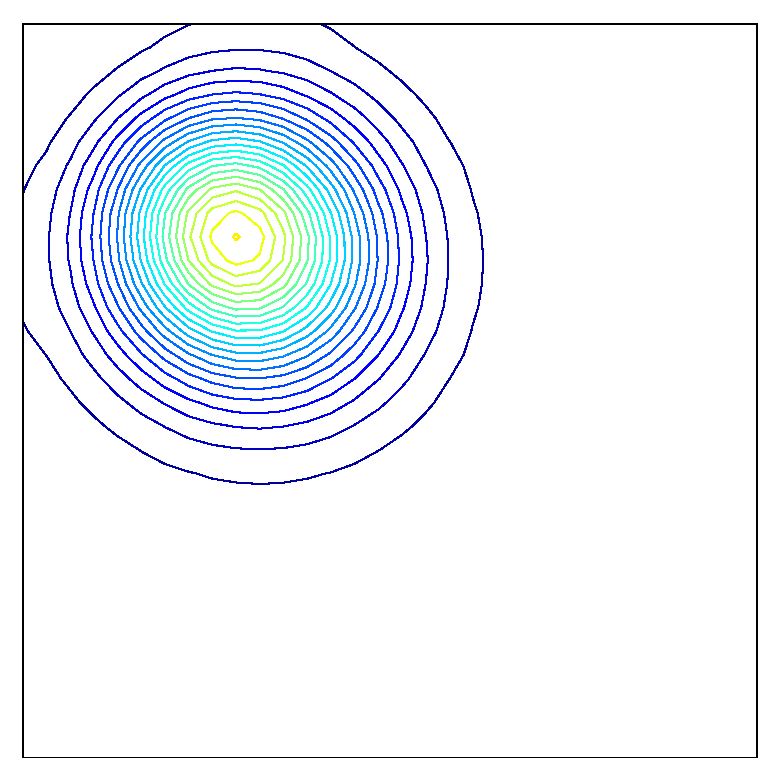
\includegraphics[width=1.6cm]{images/bump_beta/bump_beta_75_iso_05}&
\hspace{-0.45cm}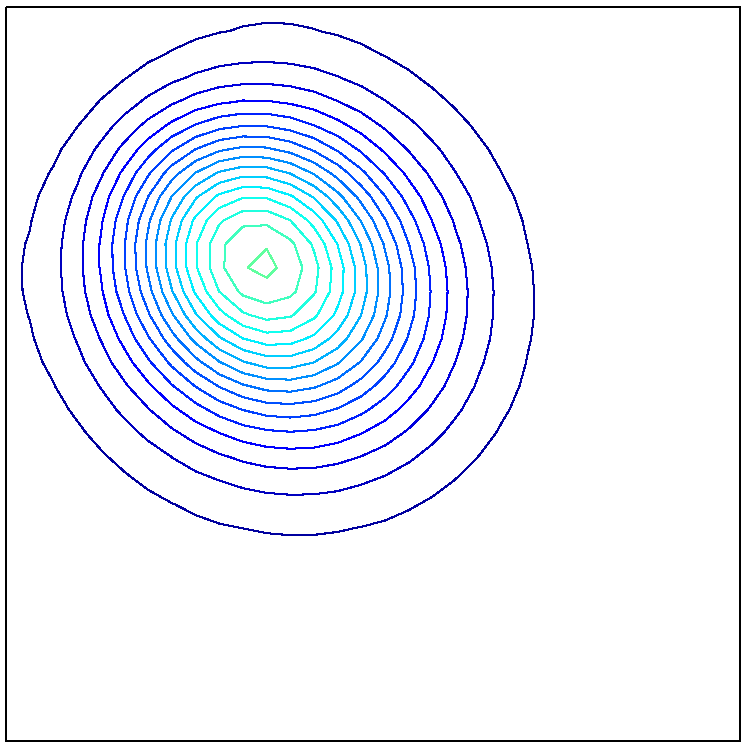
\includegraphics[width=1.6cm]{images/bump_beta/bump_beta_75_iso_09}&
\hspace{-0.45cm}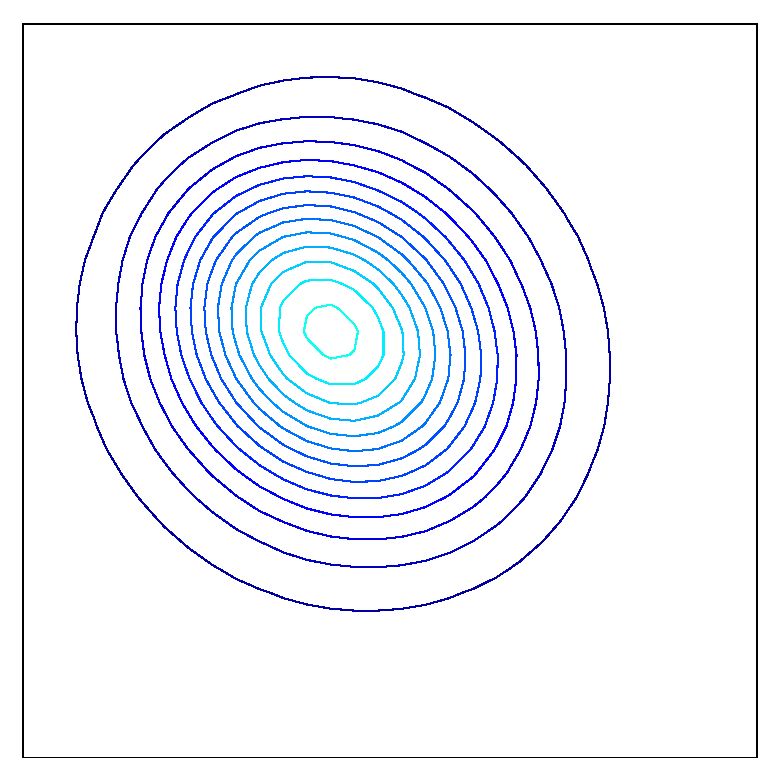
\includegraphics[width=1.6cm]{images/bump_beta/bump_beta_75_iso_13}&
\hspace{-0.45cm}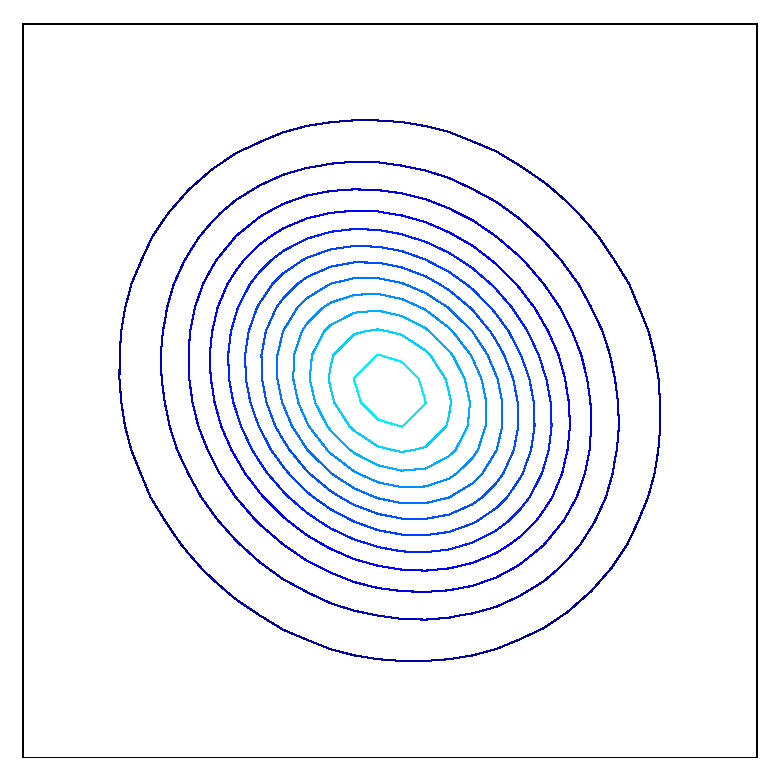
\includegraphics[width=1.6cm]{images/bump_beta/bump_beta_75_iso_17}&
\hspace{-0.45cm}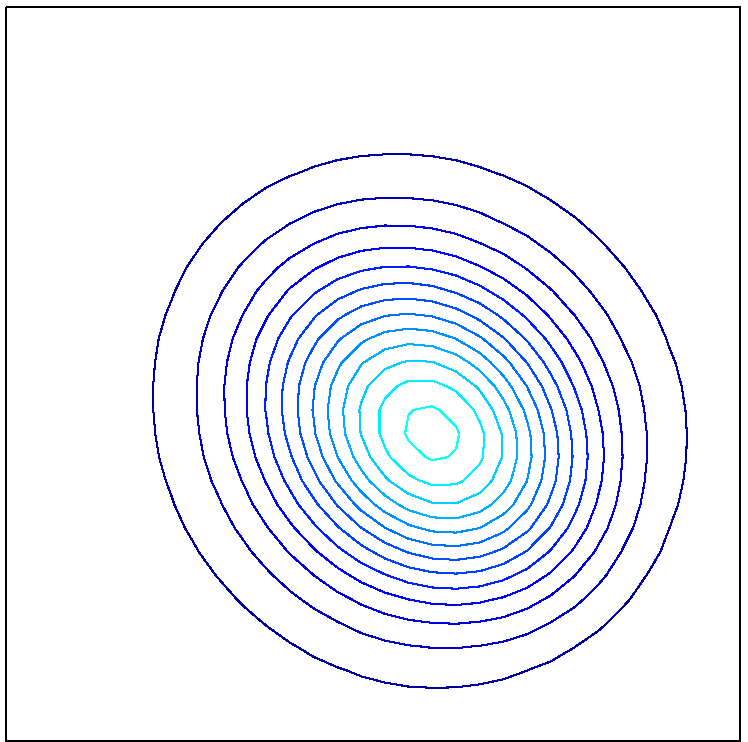
\includegraphics[width=1.6cm]{images/bump_beta/bump_beta_75_iso_21}&
\hspace{-0.45cm}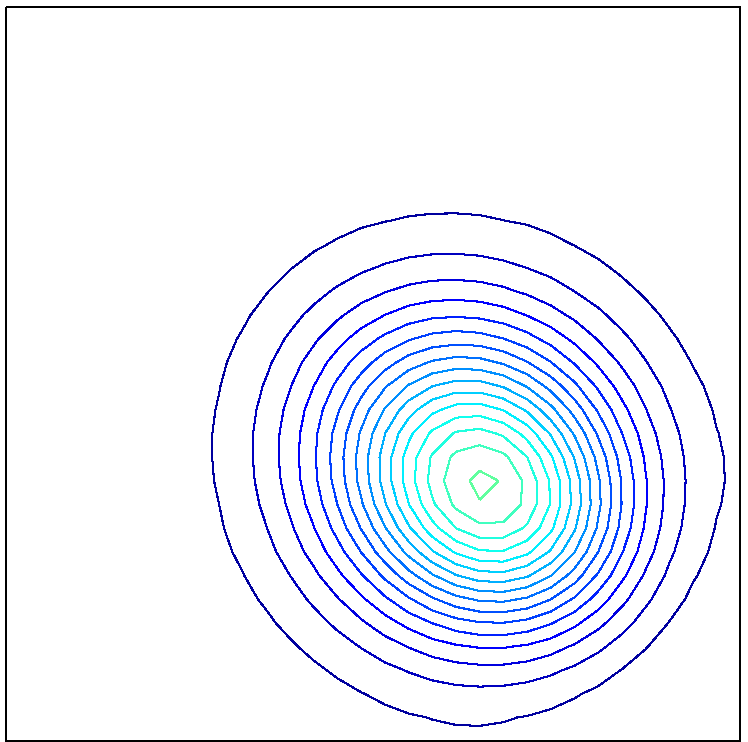
\includegraphics[width=1.6cm]{images/bump_beta/bump_beta_75_iso_25}&
\hspace{-0.45cm}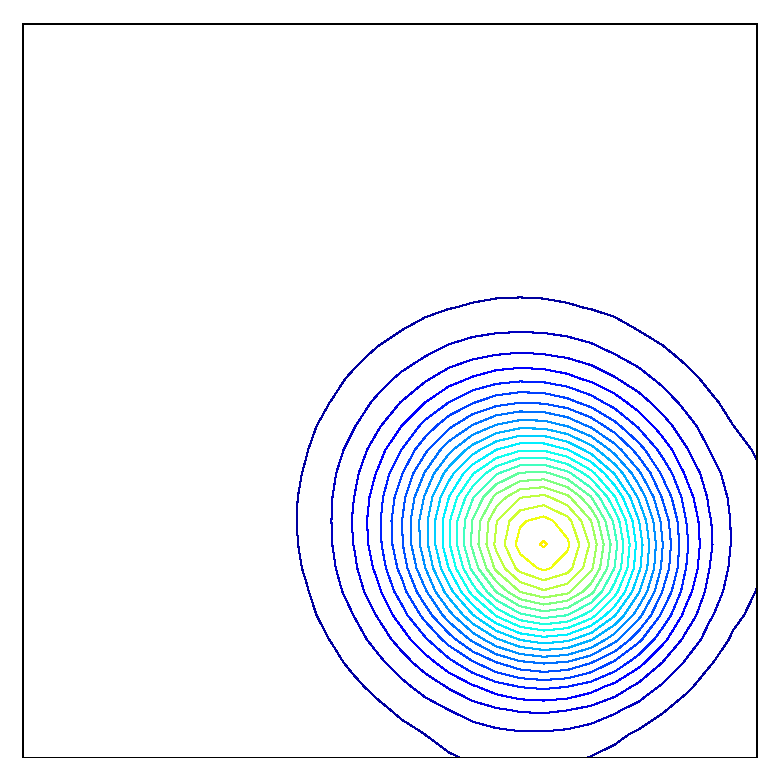
\includegraphics[width=1.6cm]{images/bump_beta/bump_beta_75_iso_29}&
\hspace{-0.45cm}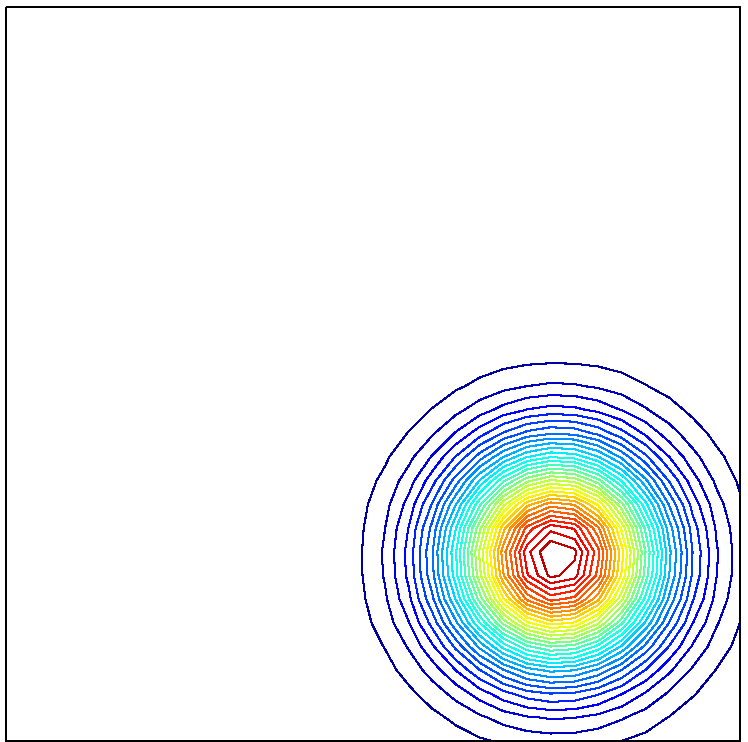
\includegraphics[width=1.6cm]{images/bump_beta/bump_beta_75_iso_33}\\
\sidecap{$\beta=1$ } &\hspace{-0.45cm}
%\animategraphics[palindrome=true,width=1.6cm]{6}{images/bump_anim/bump_beta1_iso_}{01}{33}&
%\movie[mouse=true,palindrome=true]{\includegraphics[width=1.6cm]{images/bump_beta/bump_beta1_iso_01}}{images/bump_beta/beta_1.avi}&
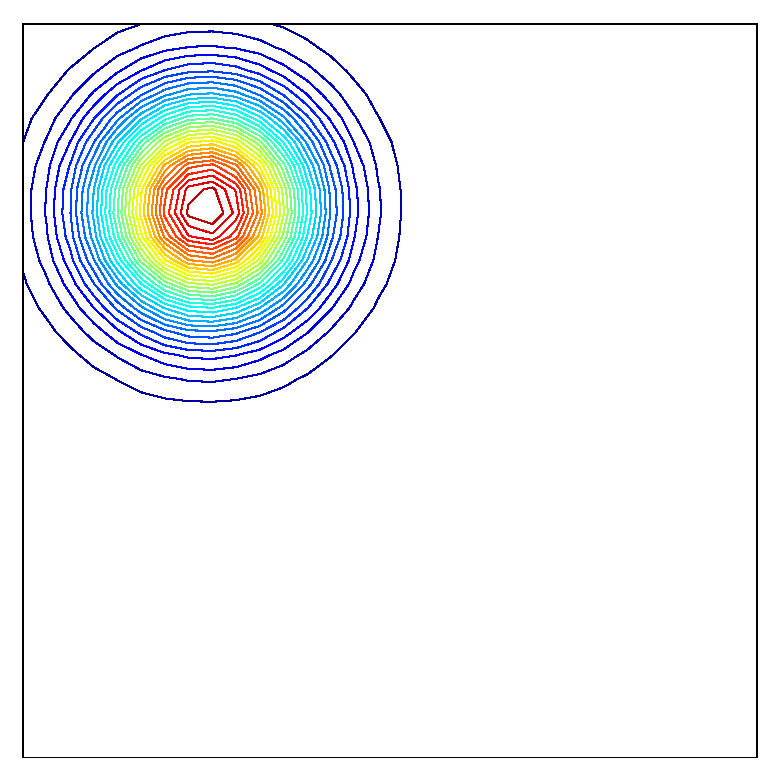
\includegraphics[width=1.6cm]{images/bump_beta/bump_beta_100_iso_01}&
\hspace{-0.45cm}\includegraphics[width=1.6cm]{images/bump_beta/bump_beta_100_iso_05}&
\hspace{-0.45cm}\includegraphics[width=1.6cm]{images/bump_beta/bump_beta_100_iso_09}&
\hspace{-0.45cm}\includegraphics[width=1.6cm]{images/bump_beta/bump_beta_100_iso_13}&
\hspace{-0.45cm}\includegraphics[width=1.6cm]{images/bump_beta/bump_beta_100_iso_17}&
\hspace{-0.45cm}\includegraphics[width=1.6cm]{images/bump_beta/bump_beta_100_iso_21}&
\hspace{-0.45cm}\includegraphics[width=1.6cm]{images/bump_beta/bump_beta_100_iso_25}&
\hspace{-0.45cm}\includegraphics[width=1.6cm]{images/bump_beta/bump_beta_100_iso_29}&
\hspace{-0.45cm}\includegraphics[width=1.6cm]{images/bump_beta/bump_beta_100_iso_33}\\
&\hspace{-0.45cm}$t=0$&\hspace{-0.45cm}$t=1/8$&
\hspace{-0.45cm}$t=1/4$&\hspace{-0.45cm}$t=3/8$&
\hspace{-0.45cm}$t=1/2$&\hspace{-0.45cm}$t=5/8$&
\hspace{-0.45cm}$t=3/4$&\hspace{-0.45cm}$t=7/8$&\hspace{-0.45cm}$t=1$\vspace{-0.2cm}
\end{tabular}
%\includegraphics[trim=100 10 100 10,clip,width=\textwidth]{./images/convergence_bump}
\caption{\label{fig:generalized_bump} 
Display of the level sets of $\iter{f}(\cdot,t)$ for several value of $t$ and $\be$ (note that for $t=0$ and $t=1$, this corresponds to $f^0$ and $f^1$).}
\end{center}
\end{figure}

Figure~\ref{fig:evol_bump_beta} shows for $\beta = 1/2$ and $\be = 3/4$ the evolution of the cost function with the iterations index $\ell$, together with the convergence of the estimate to the reference solution $(m^\star,f^\star)$ (obtained after $10^5$ iterations of the PD algorithm). We can observe that the behavior of the process with $\beta \in ]0,1[$ is different than the one observed for $\beta=1$ in Figure \ref{fig:comp_bump}. Indeed, we observe a faster convergence of the algorithms, which is consistent with the fact that $\Jfunc_\bet$ becomes more and more strongly convex as $\be$ approaches $1/2$ (see \eqref{hessian}). 

\renewcommand{\sidecap}[1]{ {\begin{sideways}\parbox{4cm}{\centering #1}\end{sideways}} }

\begin{figure}[!ht]
\begin{center}
\begin{tabular}{lccc}
\sidecap{$\beta=0.5$ } &
\hspace{-0.3cm}\includegraphics[trim=30 10 40 20,clip,width=0.31\textwidth]{images/J_beta05}&
\hspace{-0.5cm}\includegraphics[trim=30 10 40 20,clip,width=0.31\textwidth]{images/Evol_m_beta_05}&
\hspace{-0.5cm}\includegraphics[trim=30 10 40 20,clip,width=0.31\textwidth]{images/Evol_f_beta_05}\\
\sidecap{$\beta=3/4$ } &
\hspace{-0.3cm}\includegraphics[trim=30 10 40 20,clip,width=0.31\textwidth]{images/J_beta075}&
\hspace{-0.5cm}\includegraphics[trim=30 10 40 20,clip,width=0.31\textwidth]{images/Evol_m_beta_075}&
\hspace{-0.5cm}
\includegraphics[trim=30 10 40 20,clip,width=0.31\textwidth]{images/Evol_f_beta_075}\vspace{0.1cm}\\
&\hspace{-0.3cm}$\Jfunc_\bet( \iter{m},\iter{f} )$&\hspace{-0.5cm}$\norm{m^\star-\iter{m}}$&\hspace{-0.5cm}$\norm{f^\star-\iter{f}}$ \vspace{-0.2cm}
\end{tabular}
\caption{\label{fig:evol_bump_beta} At each iteration $\ell$, we plot the value of the cost function $\Jfunc_\bet(\iter{m},\iter{f})$ and the distance between the reference solution $(m^\star,f^\star)$ and the estimation $(\iter{m},\iter{f})$. The first (resp. second) row presents the result with $\beta=1/2$ (resp. $\bet=3/4$).}
\end{center}
\end{figure}

As a second example, we show in Figure~\ref{fig:generalized_MK} the different morphings obtained between pictures of Gaspard Monge and Leonid Kantorovich. The grayscale representation scales linearly between black (value of 0) and white (value of 1)  and the dimensions are $N+1=75$, $M+1=100$, $P+1=60$, $M$ being the number of discrete points in the second spatial dimension.

\renewcommand{\sidecap}[1]{ {\begin{sideways}\parbox{1.9cm}{\centering #1}\end{sideways}} }
\begin{figure}[!ht]
\begin{center}
\begin{tabular}{cccccccc}
\sidecap{$\beta=0$ } &\hspace{-0.45cm}
%\animategraphics[palindrome=true,width=1.9cm]{102}{images/MK/MK_beta0_}{01}{61}&
%\movie[mouse=true,palindrome=true]{\includegraphics[width=1.9cm]{images/MK/MK_beta0_01}}
%\includegraphics[width=1.9cm]
%{images/MK/MK_000.avi}&
\includegraphics[width=1.9cm]{images/MK/MK_beta0_01}&
\hspace{-0.35cm}\includegraphics[width=1.9cm]{images/MK/MK_beta0_11}&
\hspace{-0.35cm}\includegraphics[width=1.9cm]{images/MK/MK_beta0_21}&
\hspace{-0.35cm}\includegraphics[width=1.9cm]{images/MK/MK_beta0_31}&
\hspace{-0.35cm}\includegraphics[width=1.9cm]{images/MK/MK_beta0_41}&
\hspace{-0.35cm}\includegraphics[width=1.9cm]{images/MK/MK_beta0_51}&
\hspace{-0.35cm}\includegraphics[width=1.9cm]{images/MK/MK_beta0_61}\\
\sidecap{$\beta=0.25$ } &\hspace{-0.45cm}
%\animategraphics[palindrome=true,width=1.9cm]{12}{images/MK/MK_beta25_}{01}{61}&
%\movie[mouse=true,palindrome=true]{\includegraphics[width=1.9cm]{images/MK/MK_beta25_01}}
%\includegraphics[width=1.9cm]
%{images/MK/MK_25.avi}&
\includegraphics[width=1.9cm]{images/MK/MK_beta025_01}&
\hspace{-0.35cm}\includegraphics[width=1.9cm]{images/MK/MK_beta025_11}&
\hspace{-0.35cm}\includegraphics[width=1.9cm]{images/MK/MK_beta025_21}&
\hspace{-0.35cm}\includegraphics[width=1.9cm]{images/MK/MK_beta025_31}&
\hspace{-0.35cm}\includegraphics[width=1.9cm]{images/MK/MK_beta025_41}&
\hspace{-0.35cm}\includegraphics[width=1.9cm]{images/MK/MK_beta025_51}&
\hspace{-0.35cm}\includegraphics[width=1.9cm]{images/MK/MK_beta025_61}\\
\sidecap{$\beta=0.5$ } &\hspace{-0.45cm}
%\animategraphics[palindrome=true,width=1.9cm]{12}{images/MK/MK_beta05_}{01}{61}&
%\movie[mouse=true,palindrome=true]{\includegraphics[width=1.9cm]{images/MK/MK_beta05_01}}
%\includegraphics[width=1.9cm]
%{images/MK/MK_50.avi}&
\includegraphics[width=1.9cm]{images/MK/MK_beta05_01}&
\hspace{-0.35cm}\includegraphics[width=1.9cm]{images/MK/MK_beta05_11}&
\hspace{-0.35cm}\includegraphics[width=1.9cm]{images/MK/MK_beta05_21}&
\hspace{-0.35cm}\includegraphics[width=1.9cm]{images/MK/MK_beta05_31}&
\hspace{-0.35cm}\includegraphics[width=1.9cm]{images/MK/MK_beta05_41}&
\hspace{-0.35cm}\includegraphics[width=1.9cm]{images/MK/MK_beta05_51}&
\hspace{-0.35cm}\includegraphics[width=1.9cm]{images/MK/MK_beta05_61}\\
\sidecap{$\beta=3/4$ } &\hspace{-0.45cm}
%\animategraphics[palindrome=true,width=1.9cm]{12}{images/MK/MK_beta75_}{01}{61}&
%\movie[mouse=true,palindrome=true]{\includegraphics[width=1.9cm]{images/MK/MK_beta75_01}}
%\includegraphics[width=1.9cm]
%{images/MK/MK_75.avi}&
\includegraphics[width=1.9cm]{images/MK/MK_beta075_01}&
\hspace{-0.35cm}\includegraphics[width=1.9cm]{images/MK/MK_beta075_11}&
\hspace{-0.35cm}\includegraphics[width=1.9cm]{images/MK/MK_beta075_21}&
\hspace{-0.35cm}\includegraphics[width=1.9cm]{images/MK/MK_beta075_31}&
\hspace{-0.35cm}\includegraphics[width=1.9cm]{images/MK/MK_beta075_41}&
\hspace{-0.35cm}\includegraphics[width=1.9cm]{images/MK/MK_beta075_51}&
\hspace{-0.35cm}\includegraphics[width=1.9cm]{images/MK/MK_beta075_61}\\
\sidecap{$\beta=1$ } &\hspace{-0.45cm}
%\animategraphics[palindrome=true,width=1.9cm]{12}{images/MK/MK_beta1_}{01}{61}&
%\movie[mouse=true,palindrome=true]{\includegraphics[width=1.9cm]{images/MK/MK_beta1_01}}
%\includegraphics[width=1.9cm]
%{images/MK/MK_100.avi}&
\includegraphics[width=1.9cm]{images/MK/MK_beta1_01}&
\hspace{-0.35cm}\includegraphics[width=1.9cm]{images/MK/MK_beta1_11}&
\hspace{-0.35cm}\includegraphics[width=1.9cm]{images/MK/MK_beta1_21}&
\hspace{-0.35cm}\includegraphics[width=1.9cm]{images/MK/MK_beta1_31}&
\hspace{-0.35cm}\includegraphics[width=1.9cm]{images/MK/MK_beta1_41}&
\hspace{-0.35cm}\includegraphics[width=1.9cm]{images/MK/MK_beta1_51}&
\hspace{-0.35cm}\includegraphics[width=1.9cm]{images/MK/MK_beta1_61}\\
&\hspace{-0.45cm}$t=0$&\hspace{-0.45cm}$t=1/6$&
\hspace{-0.45cm}$t=1/3$&\hspace{-0.45cm}$t=1/2$&
\hspace{-0.45cm}$t=2/3$&\hspace{-0.45cm}$t=5/6$&
\hspace{-0.45cm}$t=1$\vspace{-0.1cm}
\end{tabular}
%\includegraphics[trim=100 10 100 10,clip,width=\textwidth]{./images/convergence_bump}
\caption{\label{fig:generalized_MK} 
Evolution of $\iter{f}(\cdot,t)$ for several value of $t$ and $\be$.
 The first and last columns represent the data $f^0$ and $f^1$. The intermediate ones present the reference solution $f^*(t)$ for successive times $t=i/6$, $i=1\cdots 5$. 
 Each line illustrates $f^*$ for different values $\beta=j/4$, $j=0\cdots 4$ of the generalized cost function. }
%{\it Please click on the first image of each line to visualize the continuous morphings}.}
\end{center}
\end{figure}


%%%%%%%%%%%%%%%%%%%%%%%%%%%%%%%%%%%%%%%%%%%%%%%%%%%%%%%%%%%%%%%%
%%%%%%%%%%%%%%%%%%%%%%%%%%%%%%%%%%%%%%%%%%%%%%%%%%%%%%%%%%%%%%%%
%%%%%%%%%%%%%%%%%%%%%%%%%%%%%%%%%%%%%%%%%%%%%%%%%%%%%%%%%%%%%%%%
\subsection{Riemannian Transportation}
\label{subsec-riemanian-examples}

We investigate in this section the approximation of a displacement interpolation for a ground cost being the squared geodesic distance on a Riemannian manifold. This is achieved by solving~\eqref{eq-optim-bb-gen} with $\be=1$ but a non-constant weight map $w$.


We exemplify this setting by considering optimal transport with obstacles, which corresponds to choosing weights $w$ that are infinity on the obstacle $\Oo \subset \RR^d \times \RR$, i.e. 
\eq{
	\foralls k \in \Gc, \quad w_k = 1 + \iota_{\Cc}(x_k,t_k) \in \{1,+\infty\}.
}
Note that the obstacles can be dynamic, i.e. the weight $w$ needs not to be constant in time. 

Figure~\ref{labyrinthe} shows a first example where $\Oo$ is a 2-D ($d=2$) static labyrinth map (the walls of the labyrinth being the obstacles, and are displayed in black). We use a $50 \times 50 \times 100$ discretization grid of the space-time domain $[0,1]^3$ and the input measures $(f^0,f^1)$ are Gaussians  with standard deviations equal to $0.04$. For Gaussians with such a small variance, this example shows that the displacement interpolation is located  closely to the geodesic path between the centers of the gaussians.


\begin{figure}[!ht]
\begin{center}
\begin{tabular}{ccccc}
%\animategraphics[palindrome=true,width=3.2cm]{12}{obstacle_mobile/bump_obstacle5_iso_0}{01}{65}&
\hspace{-0.2cm}\includegraphics[width=3cm]{images/labyrinthe/bump_obstacle5_iso_001}&
\hspace{-0.4cm}\includegraphics[width=3cm]{images/labyrinthe/bump_obstacle5_iso_012}&
\hspace{-0.4cm}\includegraphics[width=3cm]{images/labyrinthe/bump_obstacle5_iso_023}&
\hspace{-0.4cm}\includegraphics[width=3cm]{images/labyrinthe/bump_obstacle5_iso_034}&
\hspace{-0.4cm}\includegraphics[width=3cm]{images/labyrinthe/bump_obstacle5_iso_045}\\
\hspace{-0.2cm}$t=0$&
\hspace{-0.4cm}$t=1/9$&
\hspace{-0.4cm}$t=2/9$&
\hspace{-0.4cm}$t=1/3$&
\hspace{-0.4cm}$t=4/9$\\
\hspace{-0.2cm}\includegraphics[width=3cm]{images/labyrinthe/bump_obstacle5_iso_056}&
\hspace{-0.4cm}\includegraphics[width=3cm]{images/labyrinthe/bump_obstacle5_iso_067}&
\hspace{-0.4cm}\includegraphics[width=3cm]{images/labyrinthe/bump_obstacle5_iso_078}&
\hspace{-0.4cm}\includegraphics[width=3cm]{images/labyrinthe/bump_obstacle5_iso_089}&
\hspace{-0.4cm}\includegraphics[width=3cm]{images/labyrinthe/bump_obstacle5_iso_101}\\
\hspace{-0.2cm}$t=5/9$&
\hspace{-0.4cm}$t=2/3$&
\hspace{-0.4cm}$t=7/9$&
\hspace{-0.4cm}$t=8/9$&\hspace{-0.35cm}$t=1$
\end{tabular}
\caption{\label{labyrinthe} 
Evolution of $\iter{f}(\cdot,t)$ for several values of $t$, using a Riemannian manifold with weights $w_k$ (constant in time) restricting the densities to lie within a 2-D static labyrinth map.  }
\end{center}
\end{figure}


Figure~\ref{labyrinthe2} shows a more complicated setting that includes a labyrinth with moving walls: a wall appears at time $t=1/4$ and another one disappears at time $1/2$. The difference with respect to the previous example is the fact that $w$ is now time dependent. This simple modification has a strong impact on the displacement interpolation. Indeed, the speed of propagation of the mean of the density is not constant anymore since the density measure is confined in a small area surrounded by walls for $t \in [1/4,1/2]$.


\begin{figure}[!ht]
\begin{center}
\begin{tabular}{ccccc}
%\animategraphics[palindrome=true,width=3.2cm]{12}{labyrinthe4/bump_obstacle5_iso_}{001}{101}&
\hspace{-0.2cm}\includegraphics[width=3cm]{images/labyrinthe4/bump_obstacle5_iso_001}&
\hspace{-0.4cm}\includegraphics[width=3cm]{images/labyrinthe4/bump_obstacle5_iso_012}&
\hspace{-0.4cm}\includegraphics[width=3cm]{images/labyrinthe4/bump_obstacle5_iso_023}&
\hspace{-0.4cm}\includegraphics[width=3cm]{images/labyrinthe4/bump_obstacle5_iso_034}&
\hspace{-0.4cm}\includegraphics[width=3cm]{images/labyrinthe4/bump_obstacle5_iso_045}\\
\hspace{-0.2cm}$t=0$&
\hspace{-0.4cm}$t=1/9$&
\hspace{-0.4cm}$t=2/9$&
\hspace{-0.4cm}$t=1/3$&
\hspace{-0.4cm}$t=4/9$\\
\hspace{-0.2cm}\includegraphics[width=3cm]{images/labyrinthe4/bump_obstacle5_iso_056}&
\hspace{-0.4cm}\includegraphics[width=3cm]{images/labyrinthe4/bump_obstacle5_iso_067}&
\hspace{-0.4cm}\includegraphics[width=3cm]{images/labyrinthe4/bump_obstacle5_iso_078}&
\hspace{-0.4cm}\includegraphics[width=3cm]{images/labyrinthe4/bump_obstacle5_iso_089}&
\hspace{-0.4cm}\includegraphics[width=3cm]{images/labyrinthe4/bump_obstacle5_iso_101}\\
\hspace{-0.2cm}$t=5/9$&
\hspace{-0.4cm}$t=2/3$&
\hspace{-0.4cm}$t=7/9$&
\hspace{-0.4cm}$t=8/9$&\hspace{-0.35cm}$t=1$
\end{tabular}
\caption{\label{labyrinthe2} Evolution of $\iter{f}(\cdot,t)$ for several values of $t$, using a Riemannian  manifold with weights $w_k$ (evolving in time) restricting the densities to lie within a 2-D dynamic labyrinth map (i.e. with moving walls). }
\end{center}
\end{figure}


%%%%%%%%%%%%%%%%%%%%%%%%%%%%%%%%%%%%%%%%%%%%%%%%%%%%%
%%%%%%%%%%%%%%%%%%%%%%%%%%%%%%%%%%%%%%%%%%%%%%%%%%%%%
\section*{Conclusion}

In this article, we have shown how proximal splitting schemes offer an elegant and unifying framework to describe computational methods to solve the dynamical optimal transport with an Eulerian discretization. This allowed use to extend the original method of Benamou and Brenier in several directions, most notably the use of staggered grid discretization and the introduction of generalized, spatially variant, cost functions. 

%%%%%%%%%%%%%%%%%%%%%%%%%%%%%%%%%%%%%%%%%%%%%%%%%%%%%
%%%%%%%%%%%%%%%%%%%%%%%%%%%%%%%%%%%%%%%%%%%%%%%%%%%%%
\section*{Acknowledgment}

We would like to thank to Jalal Fadili for his detailed explanations of the connexion between the ADMM and DR algorithms. Nicolas Papadakis would like to acknowledge partial support from the LEFE program of INSU (CNRS). 
Gabriel Peyr\'e acknowledges support from the European Research Council (ERC project SIGMA-Vision). This work was also partially funded by the French Agence Nationale de la Recherche (ANR, Project TOMMI) under reference ANR-11-BS01-014-01.

% \fi
% \appendix
% \section{Relationship Between ADMM and DR Algorithms}

TODO: expand this. 

%%%
\subsection{ADMM}

\eq{
	\umin{x} F(x) + G \circ A(x)
}
where $A : \RR^N \rightarrow \RR^P$ injective.

Add auxiliary variable
\eq{
	\umin{x, y = Ax} F(x) + G(y)
}

Lagrangian formulation
\eq{
	\umin{x, y} \umax{u} L(x,y,u) = F(x) + G(y) + \dotp{u}{y - Ax}
}
Augmented Lagrangian formulation
\eq{
	\umin{x, y} \umax{u} L_\ga(x,y,u) = L(x,y,u)  + \frac{\ga}{2}\norm{y - Ax}^2
}
ADMM algorithm steps:
\eq{
	\iiter{x} = \uargmin{x} L_\ga(x,\iter{y},\iter{u})
}
\eq{
	\iiter{y} = \uargmin{y} L_\ga(\iiter{x},y,\iter{u})
}
\eq{
	\iiter{u} = \iter{u} + (\iiter{y} - A \iiter{x})
}
Converges for any $\ga > 0$, [Gabay, Mercier, Glowinski, Marrocco, 76]


%%%
\subsection{ADMM, prox-formulation}

Introduce the prox with the $A$ metric
\eq{
	\prox_{\ga F}^A(z) = \uargmin{x} \frac{1}{2} \norm{A x - z}^2 + \ga F(x)
}
One has
\eq{
	\prox_{\ga F}^A = A^+ \pa{ \Id - \ga \prox_{F^* \circ A^* / \ga }(\cdot/\ga) }
}
ADMM, prox formulation:
\eq{
	\iiter{x} = \prox_{F/\ga }^A ( \iter{y} - \iter{u} )
}
\eq{
	\iiter{y} = \prox_{G/\ga } ( A\iiter{x} + \iter{u} )
}
\eq{
	\iiter{u} = \iter{u} +  (\iiter{y} - A \iiter{x})
}
Advantageous if $F^* \circ A^*$ is simple. If $F \circ A$ is simple, use DR. 


%%%


Fenchel-Rockafellar duality: (here equivalent to Lagrange duality of the original problem on $(x,y)$)
\eq{
	\umin{z} F^* (-A^* z) + G^*(z)
}
DR applied to $F^* \circ -A^* + G^*$ is ADMM, but this should be understood with the correct change of variables (in particular, one cannot go back from dual to primal, one needs to use inner variables of these algorithm to perform the switch).

DR with $\al=1$:
\eq{
	\iiter{z} = \frac{1}{2} \iter{z} + \frac{1}{2} \text{RProx}_{\ga F^* \circ -A^*} \circ \text{RProx}_{\ga G^*}(\iter{z})
}
The iterates of ADMM are recovered using:
\eq{
	\iiter{x} = \prox_{F/\ga }^A ( \iter{y} - \iter{u} )
}
\eq{
	\iter{y} = \frac{1}{\ga}(\iter{z}-\iter{u})
}
\eq{
	\iter{u} = \prox_{\ga G^*}(\iter{z})
}





%%%%%%%%%%%%%%%%%%%%%%%%%%%%%%%%%%%%%%%%%%%%%%%%%%%%%
%%%%%%%%%%%%%%%%%%%REFERENCES%%%%%%%%%%%%%%%%%%%%%%%%
\bibliographystyle{plain}  % plain alpha
\bibliography{refs}		
		

\end{document}
